%    \red{Measurement of the magnitude of the collected charge has also been generally available for pixel detectors, and has been used to improve the 3D space point precision through interpolation as well as for particle identification through specific ionization measurement.
In this chapter I will present the tests performed on TJ-Monopix1 and ARCADIA-MD1; firstly I will describe the characterization of TJ-Monopix1, in terms of threshold, noise, dead time, and also provide a calibration of the output signal, and then I will show some preliminary results obtained with ARCADIA-MD1.

\section{TJ-Monopix1 characterization}
    \subsection{Threshold and noise: figure of merit for pixel detectors}
        %python3 -i calibration/scurve_tot_histo.py -f calibration/calibration_data/20220506 -i 1 100 questo script crea i file di output contenenti i gli istogrammi del tot e della s curve
        %python3 -i calibration/tot_charge_plotting.py -f calibration/calibration_data/20220506 per fare il plot della s curve e relativi residui 
        %python3 -i calibration/tot_histo2d.py -f calibration/calibration_data/PMOS/20220506 per fare l'istogramma 2d del tot           
        A characterization of threshold and noise is typically necessary since these values have an impact on the operating conditions and on the performance of the chips, so much that the signal to threshold ratio may be considered as the figure of merit for pixel detectors rather than the signal to noise ratio.
        The mean minimum stable threshold evolved through different generation of chips: in the 1st generation it was around \SI{2500}{\elementarycharge}$^-$ while in the 3rd (corresponding to nowadays chips) is less than \SI{500}{\elementarycharge}$^-$; the threshold of TJ-Monopix1 is around \SI{500}{\elementarycharge}$^-$ and is in agreement with this trend.
        Lower threshold allows for smaller signals produced in thinner sensor: from \SI{16000}{\elementarycharge}$^-$ produced in \SI{200}{\um}, the signal expected moved down to \SI{2000}{\elementarycharge}$^-$ produced in \SI{25}{\um}. 
 
        The threshold should be located between the noise peak around the baseline and the signal distribution, in particular it has to be low enough to maintain a high signal efficiency, but also high enough to cut the noise: for a low threshold many pixels can fire at the same time and a positive crosstalk feedback can set off a chain reaction eventually, causing all the other pixels to fire.
        Thus, the noise sets a lower bound to the threshold: if an occupancy $\leqslant$ $10^{-4}$ is required, for example, a probability of firing lower than that value is needed and this, assuming a gaussian noise, requires that the threshold is set at least \SI{3.7}{\sigma}, with $\sigma$ the RMS of the noise.   
        In this case, if the noise is \SI{100}{\elementarycharge}$^-$ (reasonable), the threshold must be higher than \SI[parse-numbers=false]{3.7\times100}{\elementarycharge}$^-$.\cite{Garcia-Review}
        Typically this argument sets only a minimal bound to the threshold since the variation with time and from pixel to pixel have to be taken into account: the temperature, the shift in MOSFET threshold voltage caused by radiation damage in the oxide layer and the process parameters variation across the wafer (as for example process mismatch between transistors).
            
        The noise is parameterized as Equivalent Noise Charge (ENC), which is defined as the ratio between the noise N at the output expressed in Volt and the out voltage signal S produced by \SI{1}{\elementarycharge}$^-$ entering in the preamplifier:
        \begin{equation}
            ENC\, =\, \frac{N_{out}[V]}{S_{out}[V/e-]}\,=\,\frac{V^{RMS} _{noise}}{G}
        \end{equation} 
        with G expressed in \si{V/e-}.
        Considering the threshold dispersion a requirement for the ENC is: 
        \begin{equation}
            T >\, n\,ENC \oplus T_{RMS}(x) \oplus T_{RMS}(t)
        \end{equation}
        where $T_{RMS}$ is the threshold variation during time (t) and across the matrix (x), and $n$ corresponds to the number of $\sigma$ of noise from which the threshold must set in order to obtain a firing probability lower than a certain value; taking up the example above, assuming a gaussian distribution, if n equal to 3.7, the probability that the pixel fires is less than 10$^{-4}$.

        Because of the changing of the "real" threshold, the possibility of changing and adapting the setting parameters of the FE, both in time and in space is desirable: these parameters are usually set by Digital to Analog Converter (DAC) with a number of bits in a typical range of 3-7.
        Unfortunately DAC elements require a lot of space that may be not available on the pixel area; therefore, the FE parameters are typically global, which means that they are assigned for the whole chip, or they can be assigned for regions the matrix is divided into. 
        The former case corresponds to TJ-Monopix1's design in which 7 bits are used for a total 127-DAC possible values, while the latter corresponds to the ARCADIA-MD1's one, where the number of bits depends on the particular parameter (for the threshold 6-bits DAC are used).
        Another possibility, for example implemented in TJ-Monopix2, is to allocate the space on each pixel for a subset of bits, then combining the global threshold with a fine tuning. 
        If so, the threshold dispersion after tuning is expected to decrease depending on the number of bits available for tuning:
        \begin{equation}
            \sigma_{THR, tuned} = \frac{\sigma_{THR}}{2^{n bit}}
        \end{equation}    
        where $\sigma_{thr}$ is the RMS of the threshold spread before tuning.

        To measure the threshold and noise of pixels a possible way is to make a scan varying a known charge injected through a dedicated injection capacitor: the threshold corresponds to the value where the efficiency of the signal exceeds the 50\%, and the ENC is determined from the inverse of the slope at this point.        
        Assuming a gaussian noise, e.g. a noise whose transfer function turns a voltage $\delta$ pulse in a gaussian distribution, the efficiency of detecting the signal and the noise can be described with  the function below:
        \begin{equation}
            f(x, \mu, \sigma) = \frac{1}{2} \; \left(1\,+\,erf\left(\frac{x-\mu}{\sigma \sqrt{2}}\right)\right)
            \label{eq:fit_scurve}
        \end{equation}
        where $erf$ is the error function. 
        %\begin{equation} 
        %    erf(z) = \[ \int_{0}^{z} \frac{2}{\sqrt{\pi}} e^{-x^2} dx  \]
        %\end{equation} 
        Referring to \ref{eq:fit_scurve} the threshold and the ENC corresponds to the $\mu$ and $\sigma$.
    
        I used the injection circuit available on the chip to inject 100 pulses for each input charge for a fixed threshold.
        The charge injection is realized sending a voltage step V$_{inj}$(DAC) on an injection capacitance implemented at the input of the FE circuit (Q$_{inj}$=C$_{inj}$V$_{inj}$). Knowing the nominal value of the C$_{inj}$ (\SI{230}{aF} for the PMOS flavor) one can calculate the conversion factor for the signal injected from DAC to e$^-$. 
        Since the DAC are biased at \SI{1.8}{V}, the Least significant Bit (LSB) corresponds to a voltage of \SI{14.06}{mV} from which (for the PMOS flavor) the charge for LSB \SI{1.4375}{\elementarycharge/mV} and the conversion factor therefore is \SI{20.2}{\elementarycharge/DAC}.     
        While this value is equivalent for all the PMOS flavor, the HV flavor is expected to have a different conversion factor, $\sim$ \SI{33}{\elementarycharge/DAC}, because of the different injection capacitance. 
        Besides the charge, also the duration and the period of the injection pulse can be set; it is important to make the duration short enough to have the falling edge during the dead time of the pixel (in particular during the FREEZE signal) in order to avoid the undershoot, coming at high input charge, triggering the readout and creating spurious hits. 
        Since the injection circuit is coupled in AC to the FE, if the falling edge of the pulse is sharp enough to produce an undershoot, this can be seen as a signal. 

        \begin{figure}
            \centering
            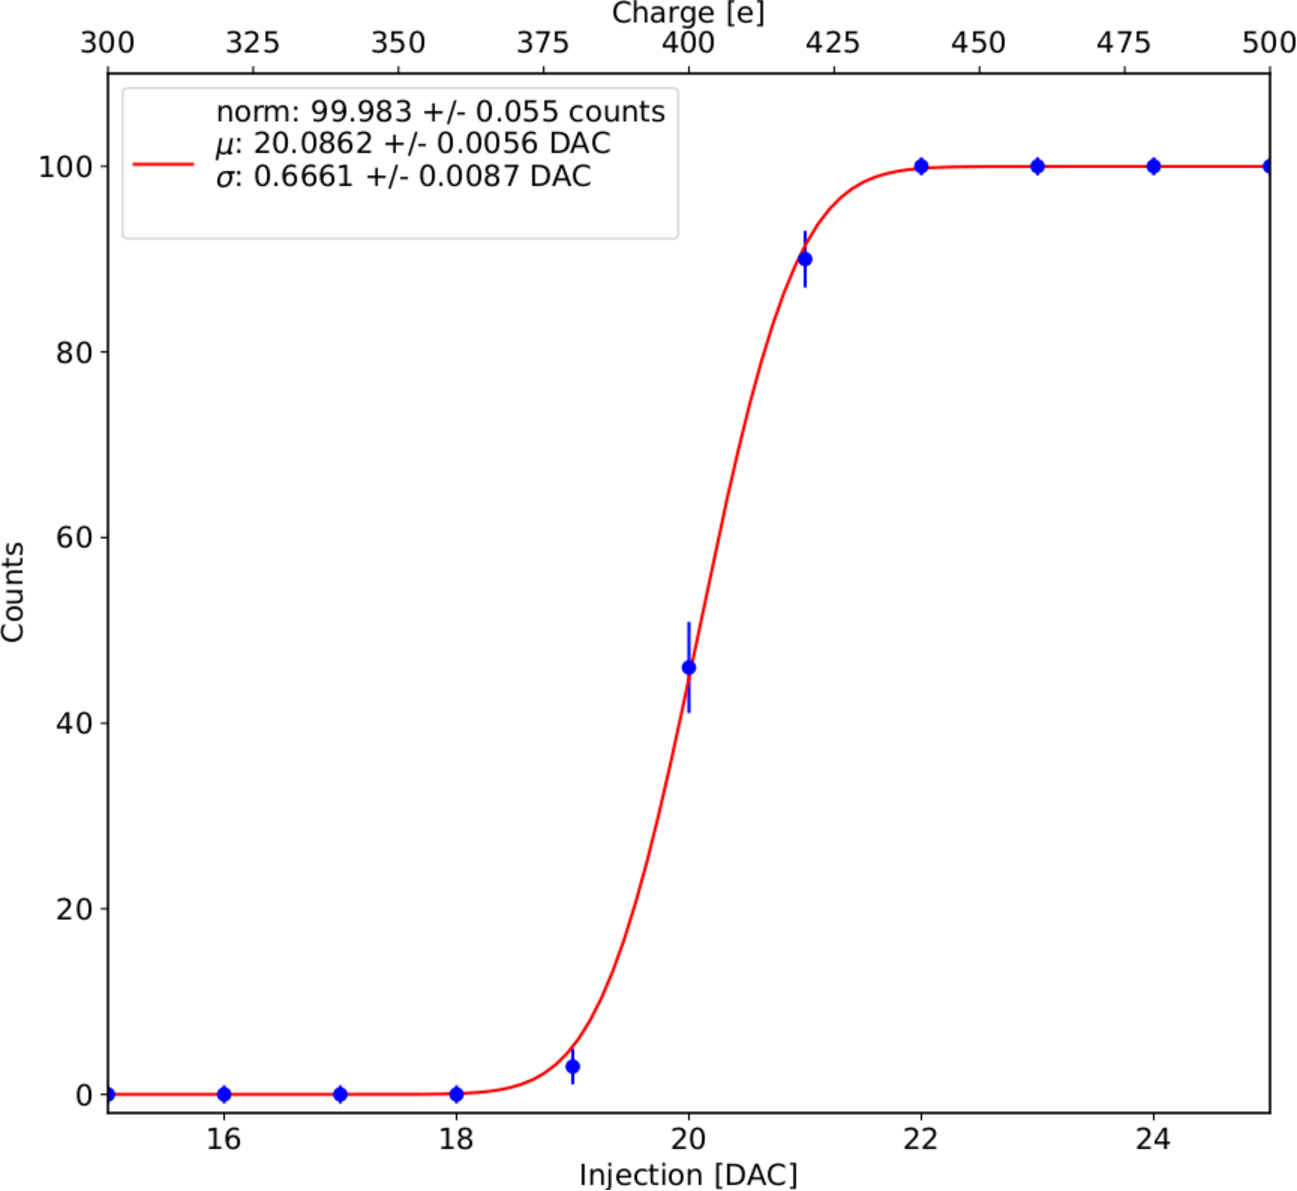
\includegraphics[width=.6\linewidth]{figures/charaterization/scurve.pdf}
            \caption{S-curve for pixel (10, 10) of the PMOS flavor (flavor B) with IDB fixed at \SI{40}{DAC}. The conversion of charge injected from DAC to electrons has been performed using a nominal conversion factor of \SI{20.3}{e-/DAC} }
            \label{fig:scurve}
        \end{figure}   

        Therefore I fitted the counts detected using the function in equation \ref{eq:fit_scurve}. Figure \ref{fig:scurve} shows an example of such fit for a pixel belonging to the flavor B with the register IDB, which sets the discriminator threshold in voltage, fixed at \SI{40}{DAC}; in figure \ref{fig:threshold_noise_hist} are shown the 1D and 2D distributions of the parameters $\mu$ and $\sigma$ of the fit found for the PMOS B flavor. Then I fitted the 1D-histograms with a gaussian function to found the average and RMS of the noise and the threshold across the matrix. The results for each flavor are reported in table \ref{tab:threshold_noise_param}; no relevant differences among the flavors have been observed regarding the noise, which results to be $\lesssim$\SI{15}{\elementarycharge}$^-$, while the threshold has been found to be $\sim$\SI{400}{\elementarycharge}$^-$ except for the PMOS C flavor, where, with the same FE settings, it is $\sim$\SI{540}{\elementarycharge}$^-$.
        \begin{figure}
            \centering
            \begin{subfigure}[b]{0.49\textwidth}
                \centering
                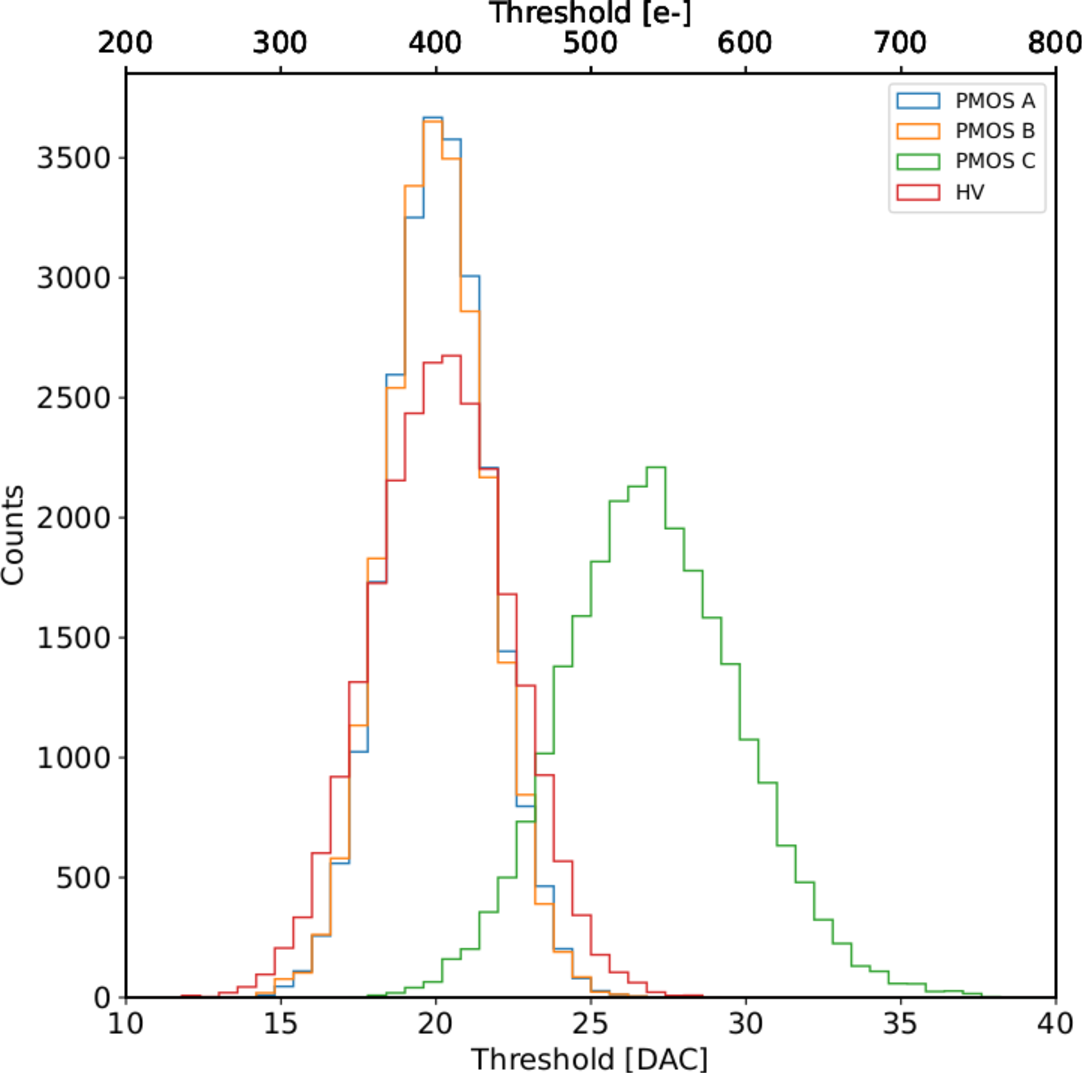
\includegraphics[width=\linewidth]{figures/charaterization/threshold_histogram.pdf}                
                \caption{Histograms of the threshold}
                \label{fig:threhsold_hist}
            \end{subfigure}
            \hfill
            \begin{subfigure}[b]{0.49\textwidth}
                \centering
                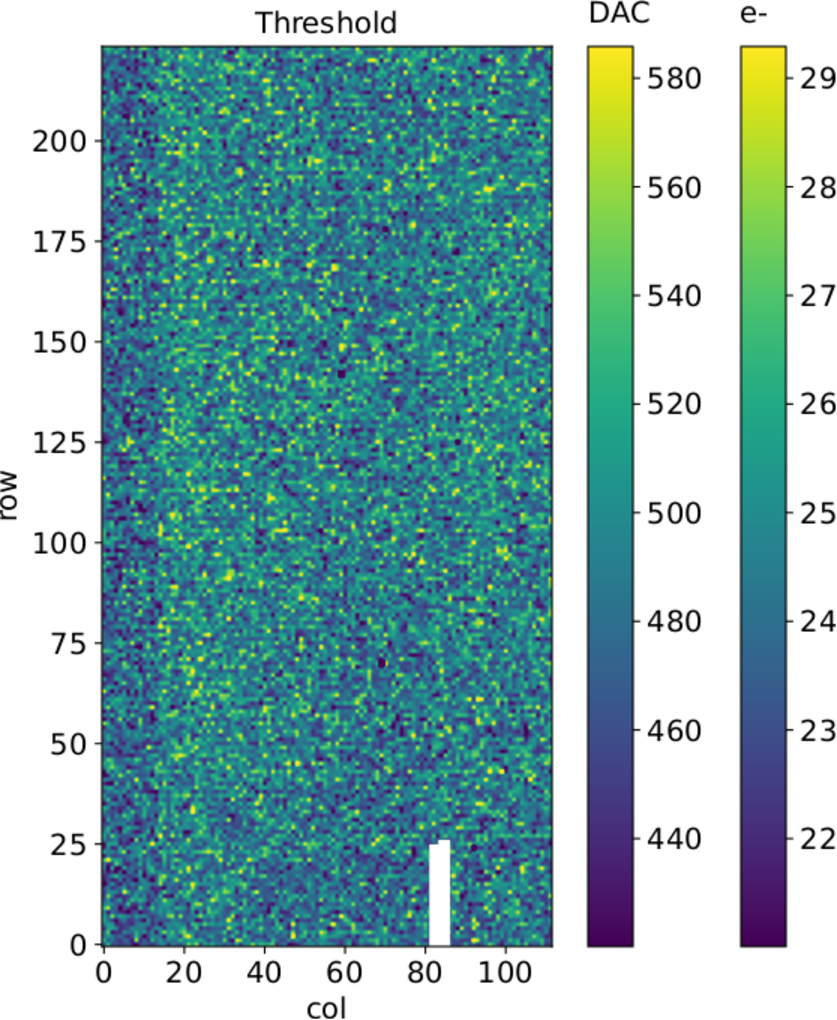
\includegraphics[width=\linewidth]{figures/charaterization/threshold_map.pdf}                
                \caption{Map of the threshold}
                \label{fig:threshold_map}
            \end{subfigure}\\ 
            \hfill
            \begin{subfigure}[b]{0.49\textwidth}
                \centering
                \includegraphics[width=\linewidth]{figures/charaterization/noise_histogram.pdf}                
                \caption{Histogram of the noise}
                \label{fig:noise_hist}
            \end{subfigure}
            \hfill
            \begin{subfigure}[b]{0.49\textwidth}
                \centering
                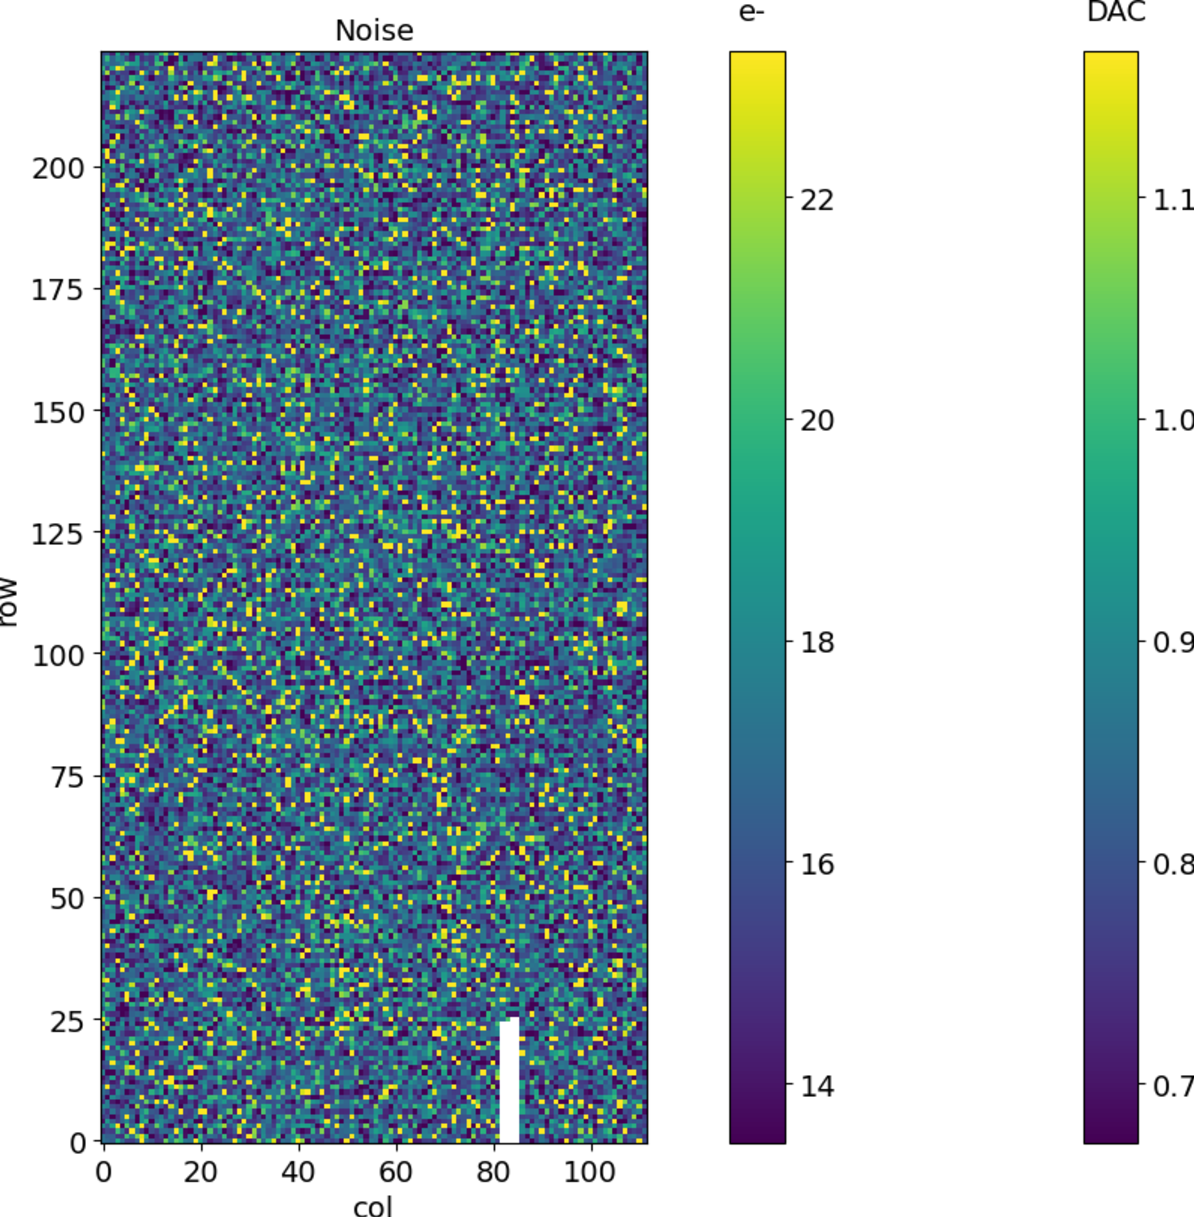
\includegraphics[width=\linewidth]{figures/charaterization/noise_map.pdf}               
                \caption{Map of the noise}
                \label{fig:noise_map}
            \end{subfigure}
            \caption{The threshold and the noise have been found fitting the s-curve of all flavor with IDB fixed at \SI{40}{DAC}. The white pixels have the injection circuit broken}
               \label{fig:threshold_noise_hist}
       \end{figure}
             
        %\begin{table}
        %        \begin{center}
        %        \begin{tabular}{| c | c | c |}
        %        \hline
        %         & DAC units & electrons \\
        %        \hline
        %        \hline
        %        Threshold        & 24.529 $\pm$ 0.049 & 511.0 $\pm$ 1.0 \\
        %        Threshold dispersion & 1.848 $\pm$ 0.033 & 36.96$\pm$0.66\\
        %        Noise            & 0.8222 $\pm$ 0.0043 & 16.444$\pm$0.086 \\
        %        Noise dispersion & 0.0975 $\pm$ 0.0030 & 1.95$\pm$0.06\\
        %        \hline
        %        \end{tabular}
        %        \caption{Flavor PMOS, IDB fixed at \SI{40}{DAC}}
        %        \label{tab:Flavor_PMOS_reser}
        %        \end{center}
        %\end{table}        

        \begin{table}[h!]
            \begin{center}
            \begin{tabular}{| c |  c | c | c |c |}
            \hline
            & PMOS A & PMOS B & PMOS C & HV \\
            \hline
            \hline
            Threshold [\si{\elementarycharge}$^-$] & 401.7$\pm$0.2 & 400.8$\pm$0.2 & 539.7$\pm$0.6 &  403.9$\pm$0.2\\
            Threshold dispersion [\si{\elementarycharge}$^-$] & 32.9$\pm$0.1 & 33.0$\pm$0.2 & 55.5$\pm$0.4 & 44.7$\pm$0.2\\
            Noise [\si{\elementarycharge}$^-$] & 13.01$\pm$0.06 & 12.26$\pm$0.07 & 13.9$\pm$0.1 & 11.7$\pm$0.1\\
            Noise dispersion [\si{\elementarycharge}$^-$] & 1.61$\pm$0.04 & 1.50$\pm$0.05 & 1.91$\pm$0.07 & 1.58$\pm$0.07\\
            \hline
            \end{tabular}
            \caption{Mean threshold and noise parameters for all flavor and their dispersion on the matrix. }
            \label{tab:threshold_noise_param}
            \end{center}
        \end{table}       
        
        %Furthermore the two portion of the chip, with FDPW and with RDPW, have been analyzed separately, because a small difference in the sensor input capacitance was expected: in fact, the deep p-well removal in the RDPW causes a small reduction of the depletion region around the collection electrode, which results in an increase of the sensor capacitance C.
        %\red{Then  , the charge to voltage conversion gain at the front-end input (Q /C ) is lower and as a result, for the same input charge a lower voltage amplitude is induced at the front-end input. }
        Although a slightly lower threshold is visible in the first biasing section (columns from 0 to 14) in the map in figure \ref{fig:threshold_map}, the threshold and noise are rather uniform across the matrix but a small systematic variation appears more evidently when using different IDB values. 
        The systematic threshold variation seems connect with the column-section and has not a well established explanation, if not a relation with the biasing group. 
        An interpretation could certainly be the transistor mismatch of the biasing DAC registers IDB and ICASN, which both adjust the effective threshold (ICASN regulates the baseline and in the presented measurement has been set at the minimum value, that is \SI{0}{DAC}).

        To verify the trend of the threshold as a function of the front end parameter IDB and find its dynamic range, I have performed different scans changing the FE register IDB. For each value I have injected the whole matrix and searched for the mean and the standard deviation of the threshold and noise distributions. The results are shown in figure \ref{fig:threshold_vs_IDB}: the blue points are the mean threshold found within the matrix, while in green is shown the width (threshold $\pm$ trhreshold dispersion) of the threshold distribution, i.e. the threshold dispersion. 
        While the threshold increases at higher IDB, the ENC decreases of $\sim$\SI{4}{\elementarycharge}$^-$,which is $\sim$1/3 of the noise at IDB=\SI{40}{DAC}. \red{Ma ora che ci penso forse del noise ci dovrei mettere un plot? }
        \begin{figure}[h!]
            \centering
            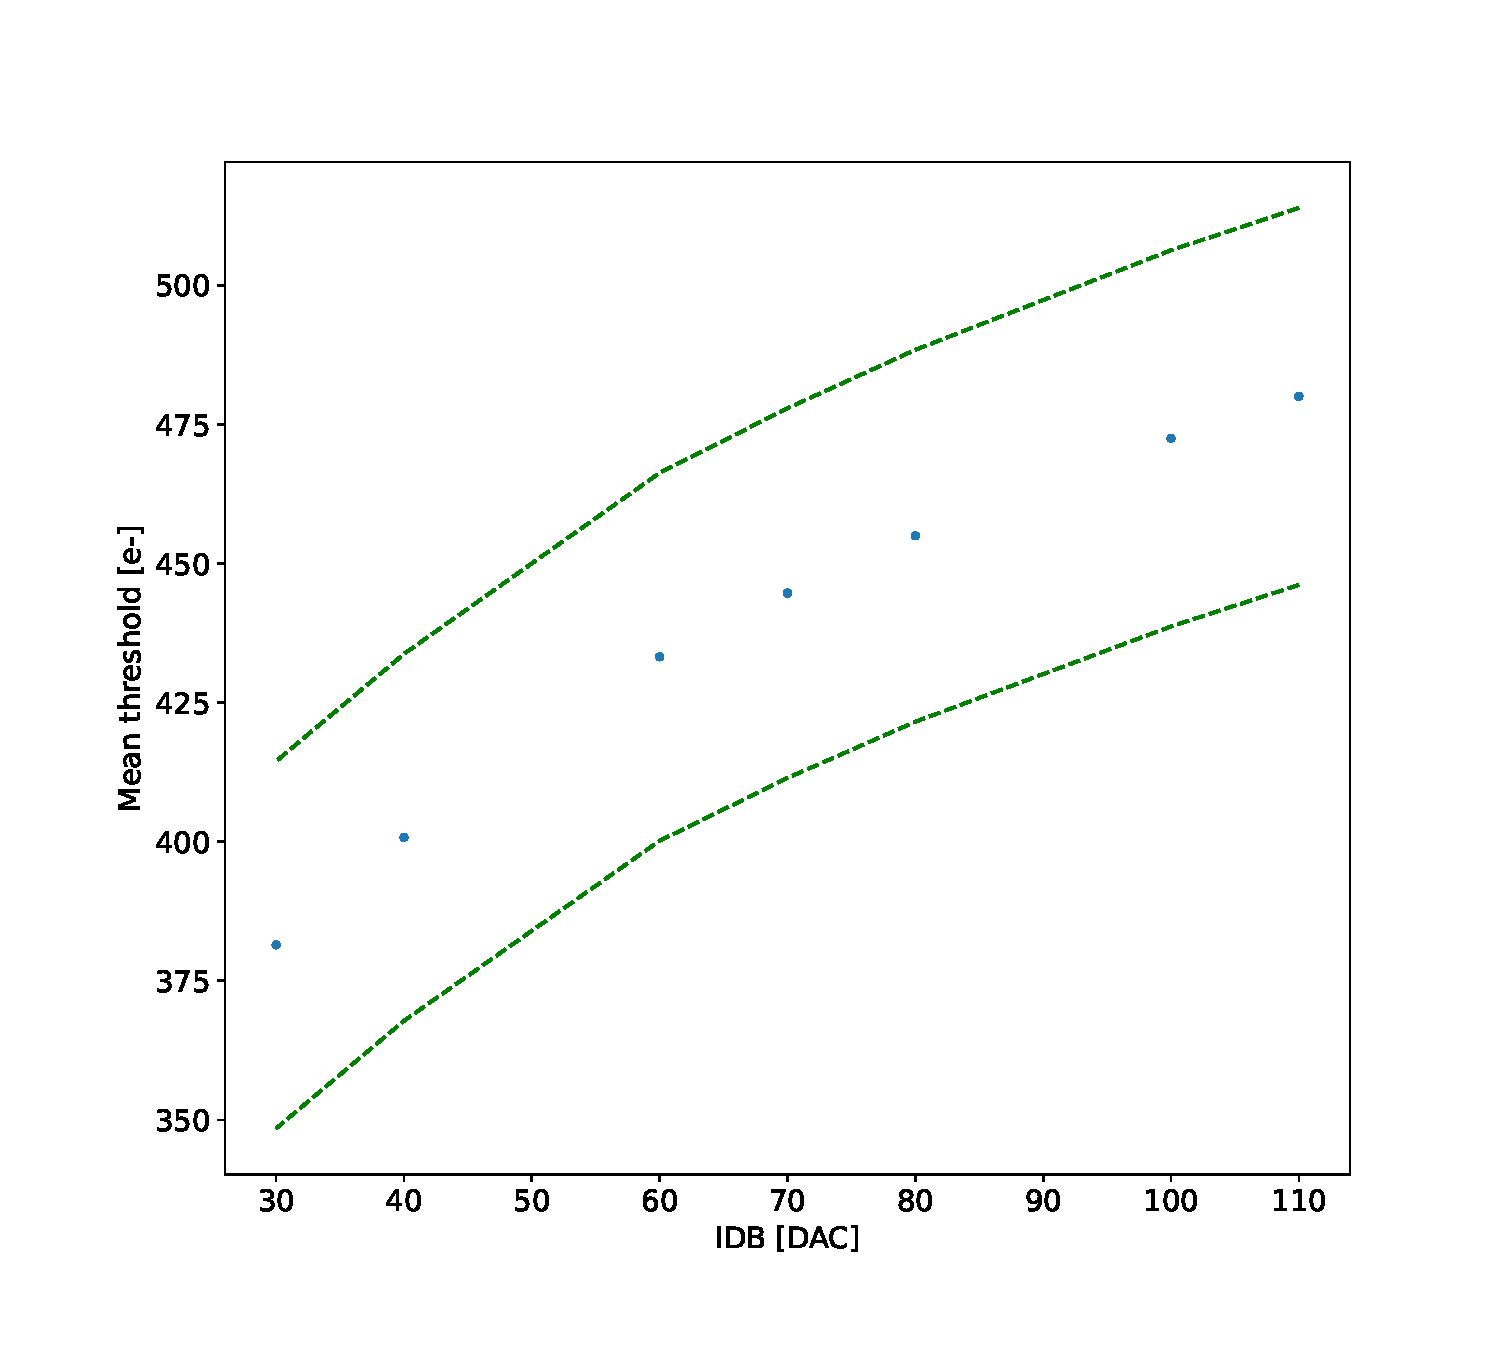
\includegraphics[width=.70\linewidth]{figures/charaterization/thr_vs_IDB.pdf}
            \caption{Flavor PMOS (B) with Psub-Pwell biased at -\SI{6}{V}. Threshold converted in electrons (using the nominal conversion factor \SI{20.2}{\elementarycharge/DAC}) vs the register which sets the threshold, IDB.  }
            \label{fig:threshold_vs_IDB}
        \end{figure}            
        Then, to evaluate the operation and the occupancy of the chip at different threshold I have checked how the number of pixel masked changes with the threshold (fig.\ref{fig:noisy_pixels}). The masking algorithm I have used search for pixels with rate $>$\SI{10}{Hz} and mask them. In our standard condition a very low noise hit rate of $\sim$\SI{3}{Hz} is intentionally achieved masking a dozen of pixels on the whole flavor.
        \begin{figure}[h!]
            \centering
            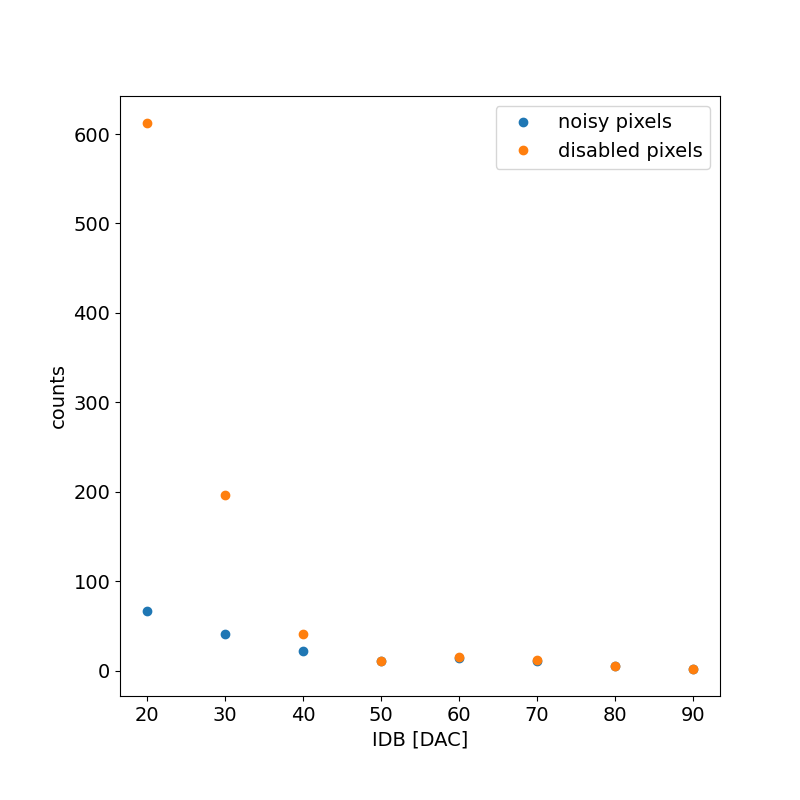
\includegraphics[width=.6\linewidth]{figures/charaterization/noisy.png}
            \caption{Number of pixels masked at different IDB: beacuse of the algorithm for masking not all the pixels masked are noisy. In blue the number of noisy pixels, while in orange the number of pixels disabled}
            \label{fig:noisy_pixels}
        \end{figure}   


    \subsection{Linearity of the ToT}
        %python3 -i acquisition_Fe55/fit_tot_single_pixel.py -f acquisition_Fe55/source_PMOSS/ per fare il fit    
        %python3 -i acquisition_Fe55/plot_tot_single_pixel.py -f acquisition_Fe55/source_PMOSS/ -fl 'gauss_line' per fare il plot di single pixel
        I have already stated in chapter \ref{chap:Monopix_Arcadia} that TJ-Monopix1 returns an output signal proportional to the charge released by a particle in the epitaxial layer, which is the Time over Threshold; the ToT is saved as a 6-bit variable and therefor its dynamic range is 0-64, which corresponds to \numrange[range-phrase = --]{0}{1.6}\si{\us} assuming a clock frequency of \SI{40}{MHz}.
        When a pulse is longer than \SI{1.6}{\us} the counter rolls back to zero and there is no way to distinguish that charge from a lower one with the same ToT: that is the rollover of the ToT (fig.\ref{fig:ToT_histo2d}).   

        In order to associate the ToT (in range 0-64) to the charge, a calibration of the signal is necessary. The output of TJ-Monopix1 is approximately a triangular pulse, resulting in a linear relationship between ToT and charge: 
        \begin{equation}
            Q\, [DAC] = \frac{(ToT\,[au]\, -\, offset\,[au])}{slope\, [au/DAC]} 
        \end{equation}\label{eq:calibration}
        where $slope$ and $offset$ are the fitted parameters of the calibration.
        It is important to keep in mind that the main application target of TJ-Monopix1 is in the inner tracker detector of HEP experiments, then the main feature is the efficiency, then a rough calibration of the signal to charge is fine. The ToT information can be used both to better reconstruct the charge deposition in cluster in order to improve the track resolution, and for particle identification, through $\frac{dE}{dx}$, especially for low momentum particles which do not reach the dedicated detectors.
                        
        The study of the output signal has been possible via the injection: I fitted the ToT versus the pulse amplitude injected for all the pixels within the matrix.
        In figure \ref{fig:ToT_vs_charge} there is an example of fit for a pixel belonging to the flavor B, while in figure \ref{fig:ToT_histograms} there are the histograms and the maps of the parameters of the line-fit for all flavors with IDB fixed at \SI{40}{DAC}. Here a difference among the biasing section appears: since the slope of the ToT is related to the gain of the preamplifier (increasing the gain also increases the ToT), the mismatch is probably due to the transistor contributing to the amplification stage.

        I fitted the average ToT of all the pulses recorded as a function of the pulse amplitude; data affected by rollover have been removed in order to avoid introducing a bias in the mean values.
        In figure \ref{fig:ToT_vs_charge} are shown both the fits with a line (red) and with a second order polynomial (green): at the bounds of the ToT range values deviate from the line model. Since the deviation is lower than 1\% and it only interests the region near the 0 and the 64, in first approximation it is negligible. 
        \begin{figure}
            \centering
            \begin{subfigure}[b]{0.49\textwidth}
                \centering
                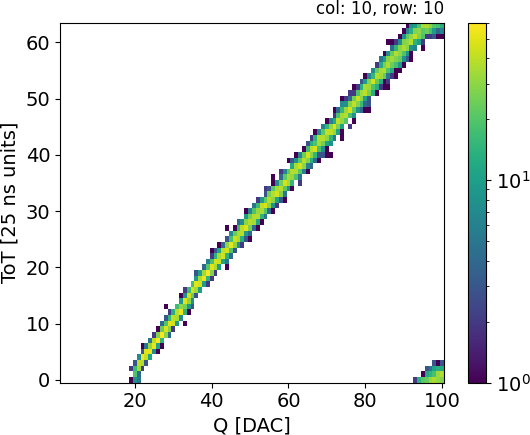
\includegraphics[width=\linewidth]{figures/charaterization/ToT_rollover.png}                 
                \caption{}
                \label{fig:ToT_histo2d}
            \end{subfigure}
            \hfill
            \begin{subfigure}[b]{0.49\textwidth}
                \centering
                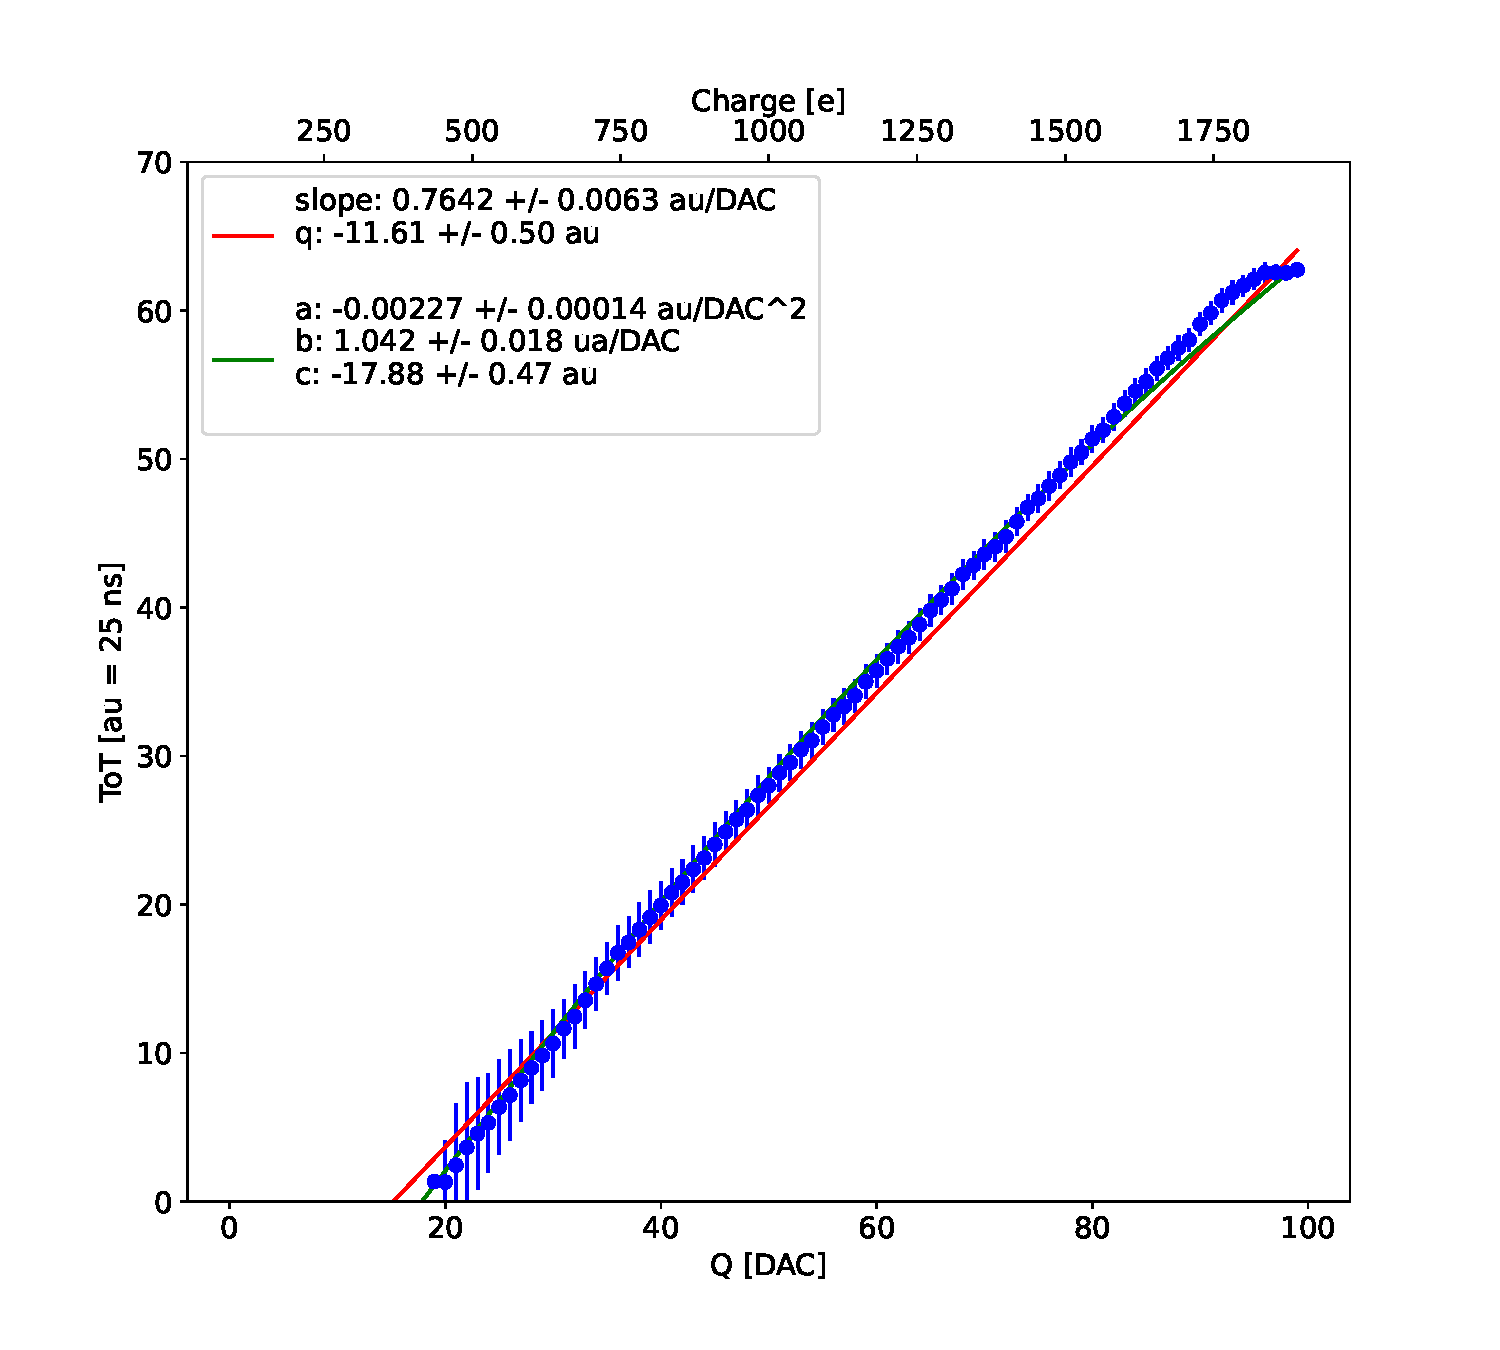
\includegraphics[width=\linewidth]{figures/charaterization/ToT_injection.pdf}             
                \caption{}
                \label{fig:ToT_vs_charge}
            \end{subfigure}
            \caption{The figures refer to pixel (10, 10) of the PMOS-reset flavor B with IDB fixed at \SI{40}{DAC}.
            (a) Histogram of the injection pulses: the ToT is in range 0-64 since it is represented by 6 bit, so when achieving the 64 it rolls over back to the zero. (b) Mean ToT vs the the charge: the mean has been calculated removing the rollover hits.}
            \label{fig:ToT}
       \end{figure}
   
       \begin{figure}
        \centering
        \begin{subfigure}[b]{0.49\textwidth}
            \centering
            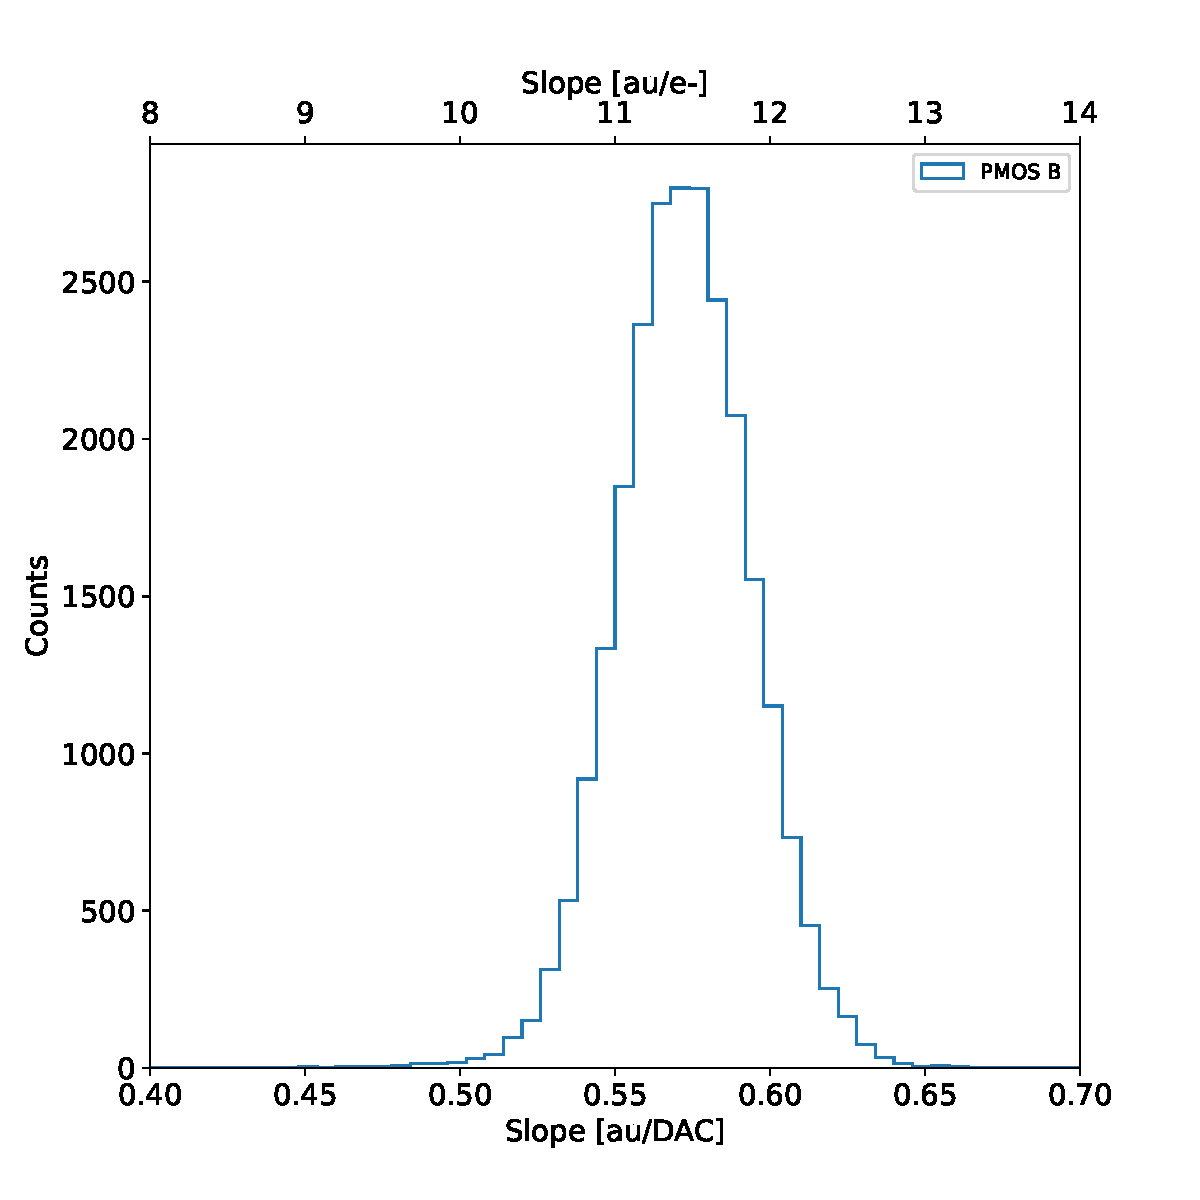
\includegraphics[width=\linewidth]{figures/charaterization/slope_histogram.pdf}
            \caption{}
            \label{fig:slope_histo}
        \end{subfigure}
        \hfill
        \begin{subfigure}[b]{0.49\textwidth}
            \centering
            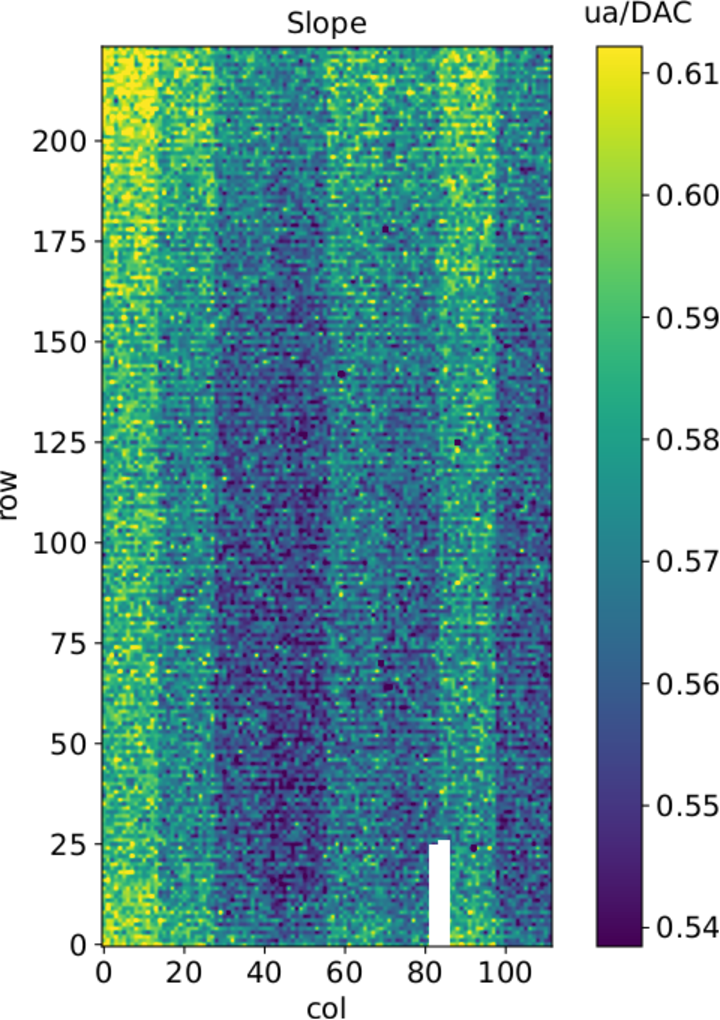
\includegraphics[width=\linewidth]{figures/charaterization/slope_map.pdf}
            \caption{}
            \label{fig:slope_map}
        \end{subfigure}\\
        \begin{subfigure}[b]{0.49\textwidth}
            \centering
            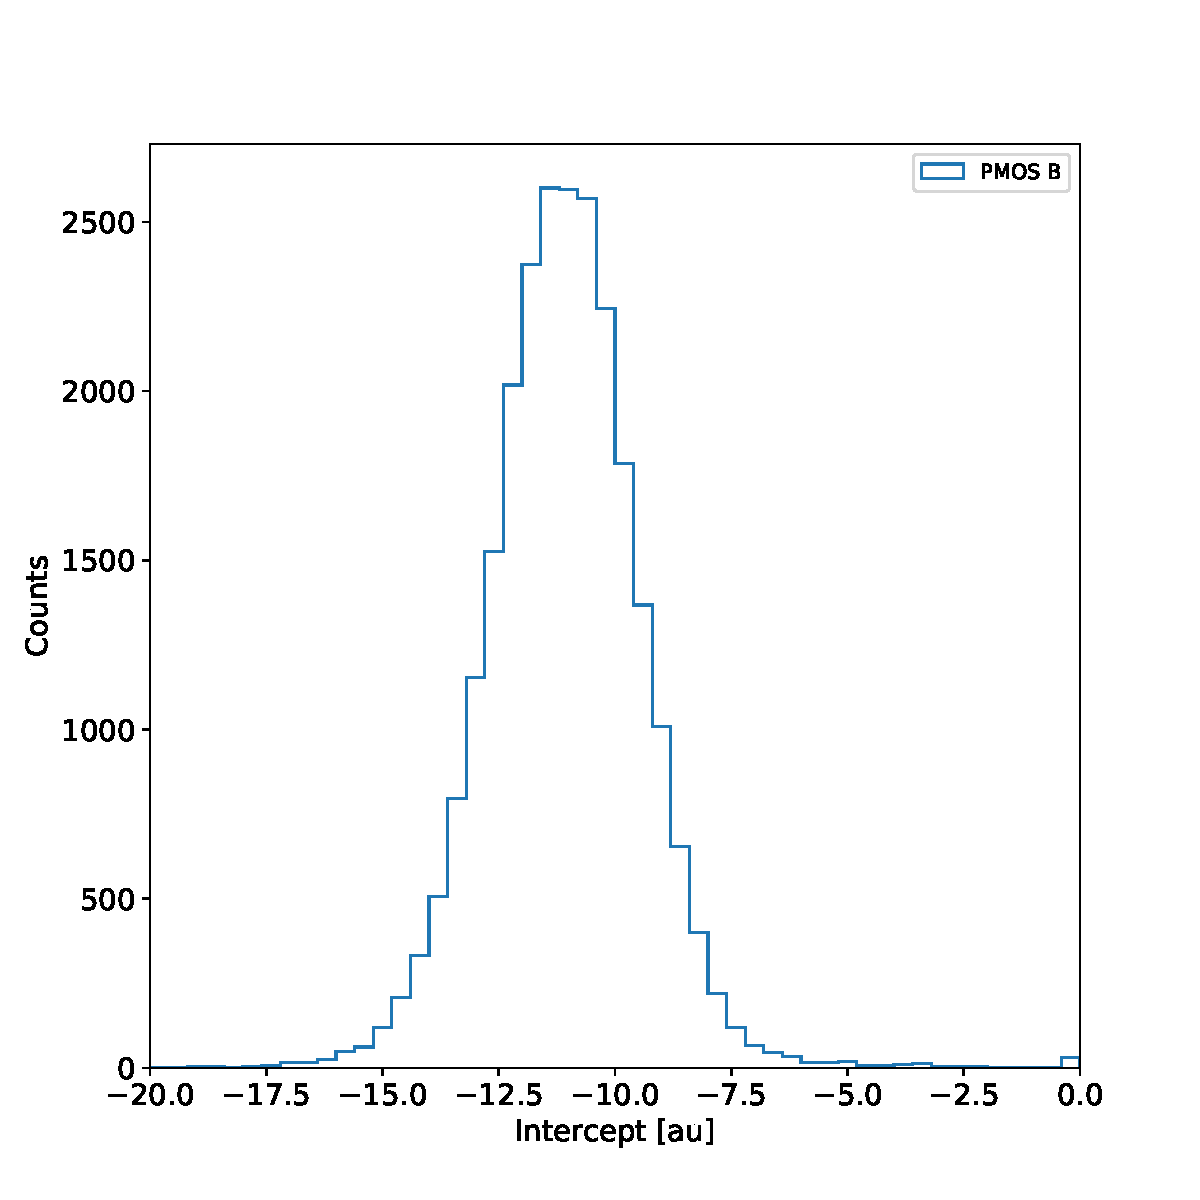
\includegraphics[width=\linewidth]{figures/charaterization/intercept_histogram.pdf}
            \caption{}
            \label{fig:offset_histo}
        \end{subfigure}
        \hfill
        \begin{subfigure}[b]{0.49\textwidth}
            \centering
            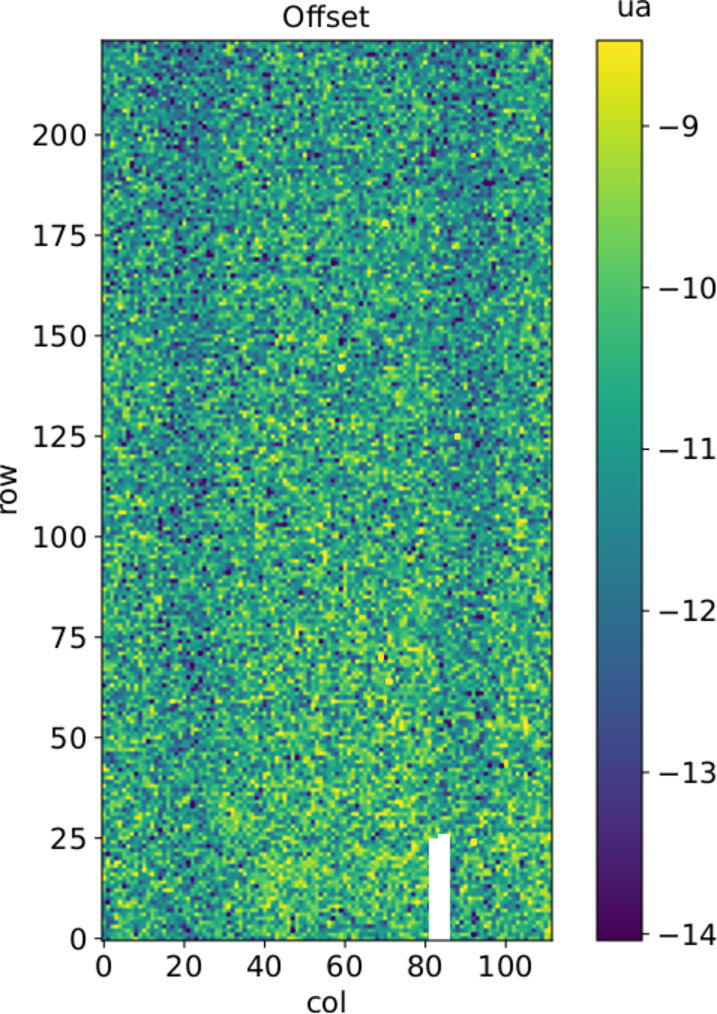
\includegraphics[width=\linewidth]{figures/charaterization/offset_map.pdf}          
            \caption{}
            \label{fig:offset_map}
        \end{subfigure}
        \caption{Histograms of the calibration parameters, slope (a) and offset (b), found fitting the ToT with a line, for the flavor B and with IDB fixed at \SI{40}{DAC}. Maps of the calibration parameters, slope (a) and offset (b), found fitting the ToT with a line, with IDB fixed at \SI{40}{DAC}.}
           \label{fig:ToT_histograms}
   \end{figure}
        
    \subsection{Calibration of the ToT}\label{sec:cal_ToT}
    %python3 -i acquisition_Fe55/fit_tot_single_pixel.py -f acquisition_Fe55/source_PMOSS/Fe_acquisitions_6V/ per fare i fit. Attenzione che prende i file degli istogrammi npz già    
        For the calibration of the Time over Threshold signal I have used both the injection and a radioactive source in order to fix an absolute scale of the charge detected. 
        The calibration is based on the following assumptions:
        \begin{itemize}
            \item \SI{0}{DAC} corresponds to \SI{0}{\elementarycharge}$^-$
            \item a ToT of \SI{1}{clock} count corresponds to a charge produced in the bulk equal to the threshold  
        \end{itemize}
        \begin{figure}
            \centering
            \begin{subfigure}[b]{0.49\textwidth}
                \centering
                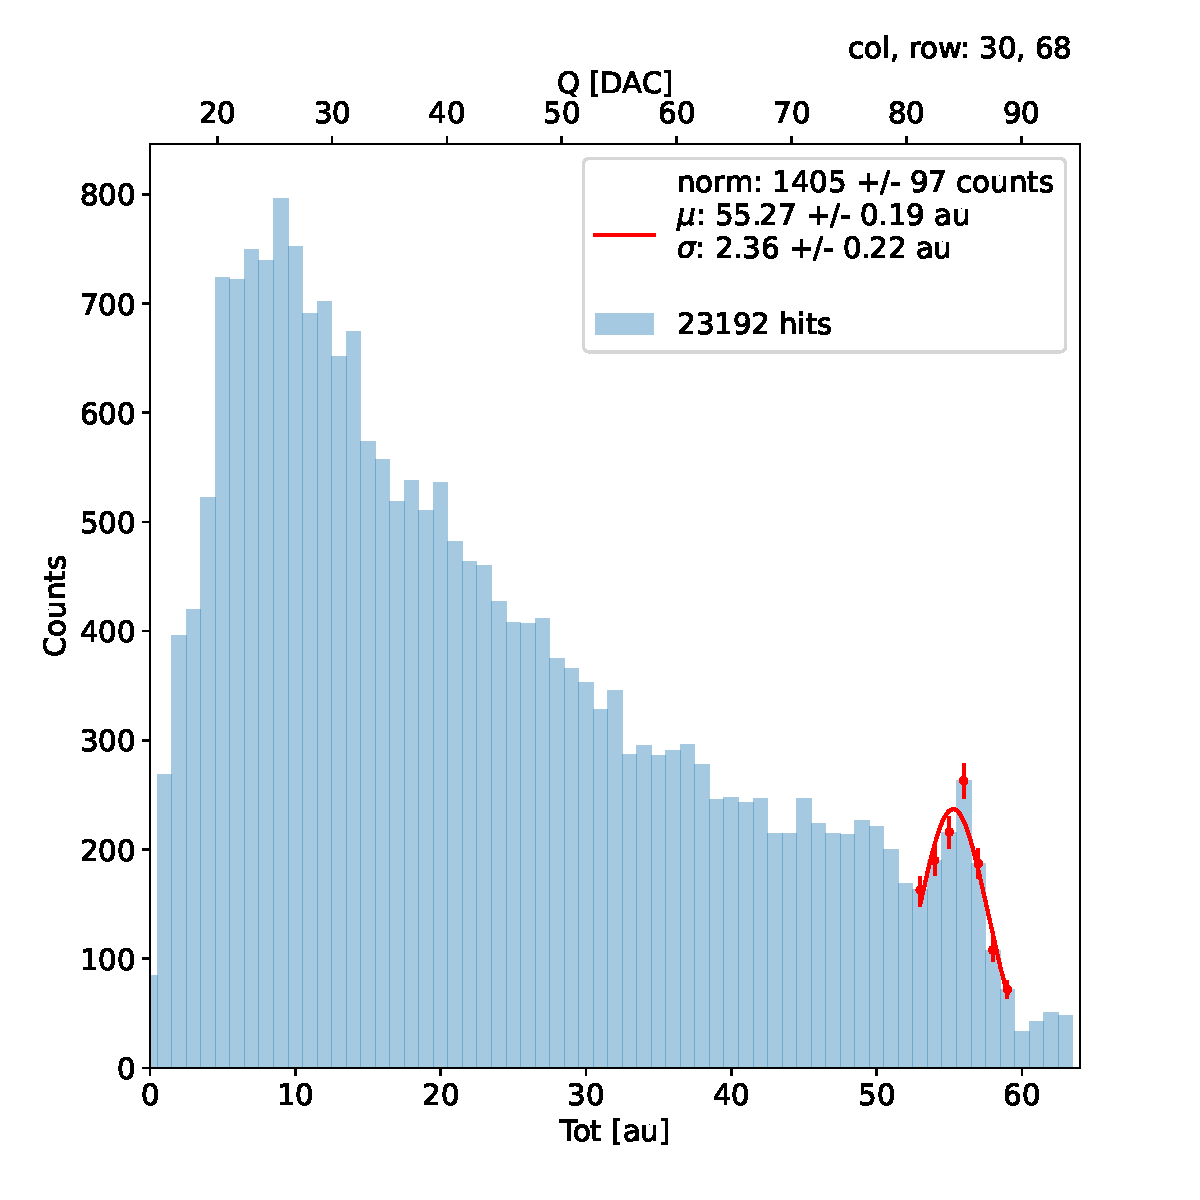
\includegraphics[width=\linewidth]{figures/charaterization/fit_gauss_r69.pdf}
                \caption{}
                \label{fig:gauss_c68}
            \end{subfigure}
            \hfill
            \begin{subfigure}[b]{0.49\textwidth}
                \centering
                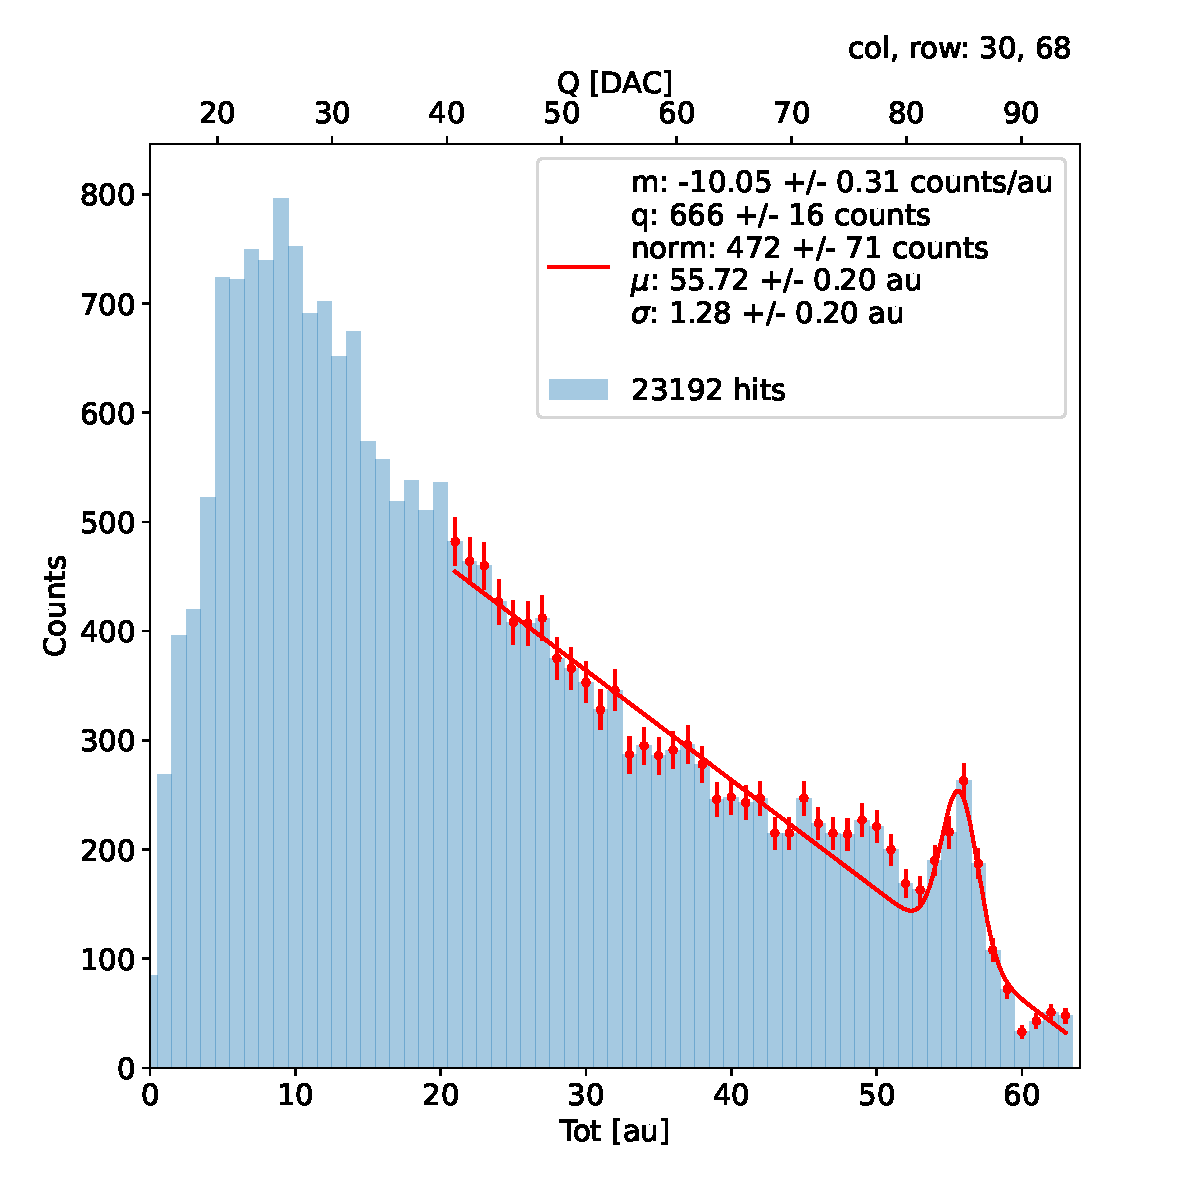
\includegraphics[width=\linewidth]{figures/charaterization/fit_line_gauss_r69.pdf}
                \caption{}
                \label{fig:gauss_line_c68}
            \end{subfigure}\\
            \begin{subfigure}[b]{0.49\textwidth}
                \centering
                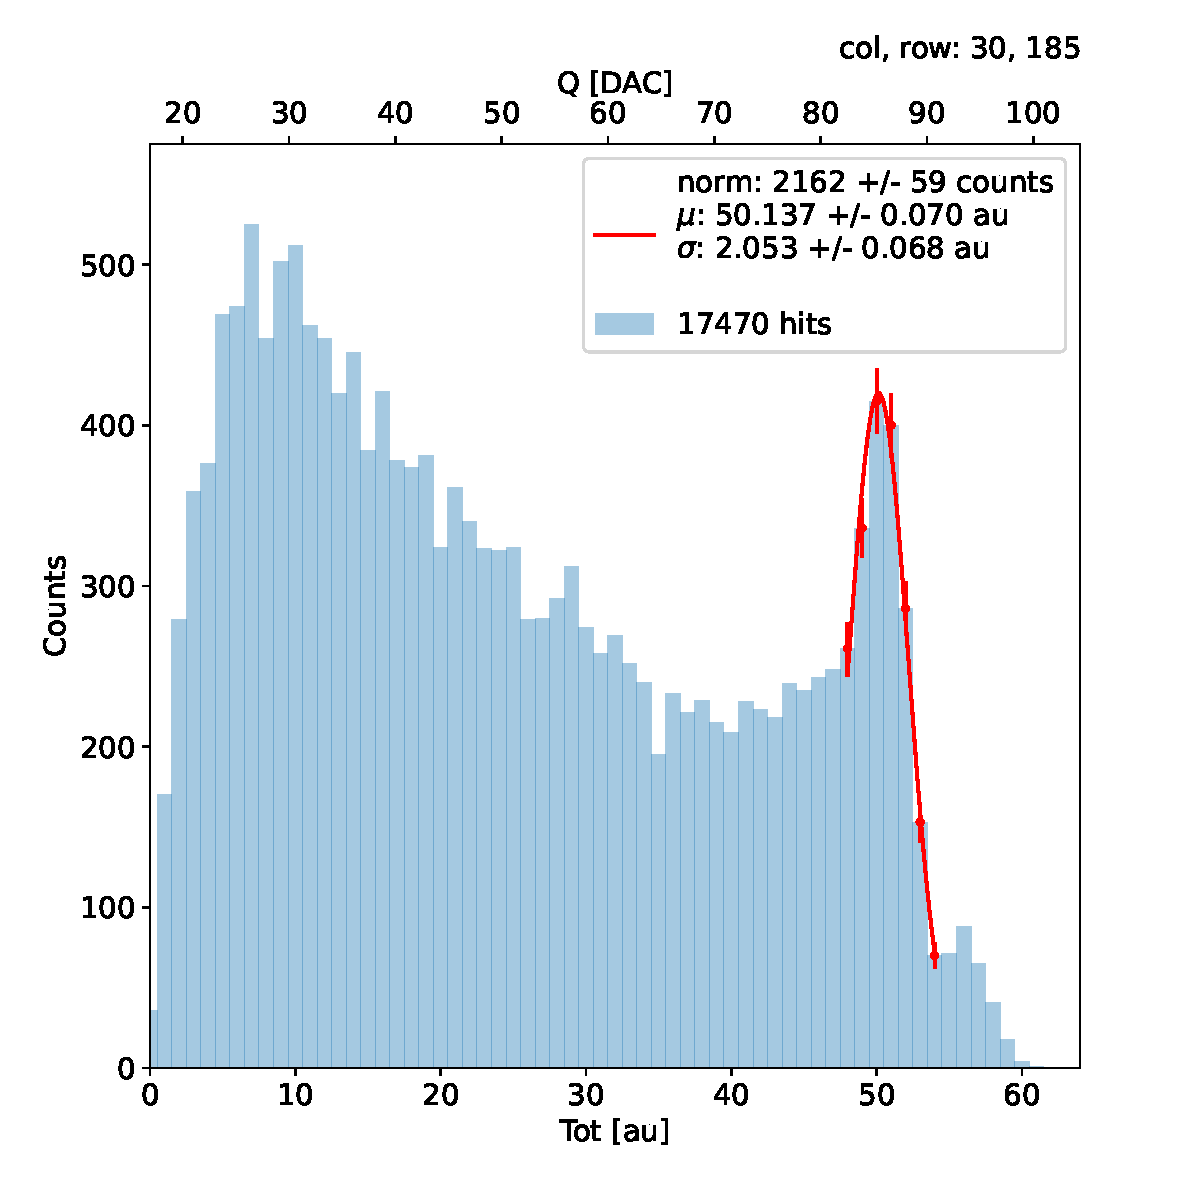
\includegraphics[width=\linewidth]{figures/charaterization/fit_gauss_r185.pdf}
                \caption{}
                \label{fig:gauss_c185}
            \end{subfigure}
            \hfill
            \begin{subfigure}[b]{0.49\textwidth}
                \centering
                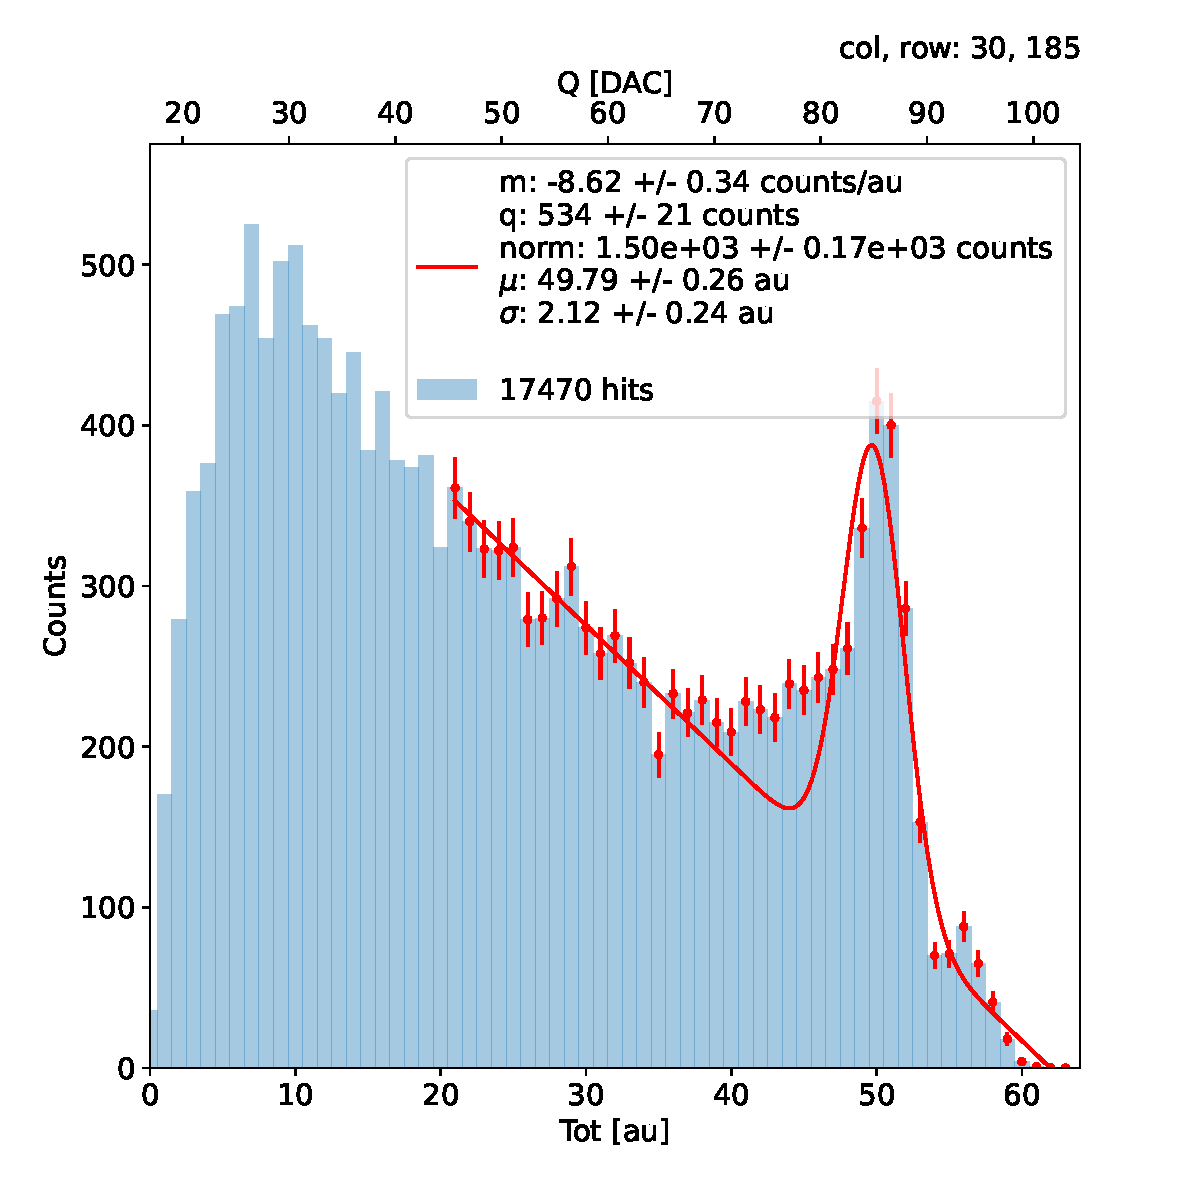
\includegraphics[width=\linewidth]{figures/charaterization/fit_line_gauss_r185.pdf}      
                \caption{}
                \label{fig:gauss_line_c185}
            \end{subfigure}
            \caption{Both strategies \ref{eq:gauss} and \ref{eq:gauss_line} of fitting the Fe55 peak are shown for two pixels on the matrix: the (a) and (b) refers to pixel (30, 68) which has a FDPW, while the (c) and (d) refers to pixel (30, 185) which has a RDPW. The fit has been performed using the bins colored by red.}
            \label{fig:Fe55_spectrum_pixels}
       \end{figure}
        Considering that the charge injected in the FE depends on the value of the C$_{inj}$ (Q$_{inj}$=C$_{inj}$V$_{inj}$) which is different from pixel to pixel, the true charge injected does not correspond to the nominal value expected assuming C$_{inj}$=\SI{230}{aF}.
        Accordingly to that, a measurement of the injection capacitance provides both an absolute calibration of C$_{inj}$ and a conversion factor K to have a correspondence of the DAC signal in electrons. 
        K and C$_{inj}$ are defined respectively as:
        \begin{equation}
            K\, [\si{\elementarycharge}^-/\si{DAC}] = \frac{1616\,[\si{\elementarycharge}^-]}{Q\,[\si{DAC}]}
        \end{equation}
        \begin{equation}
            C_{inj}\,[\si{F}] =\, K\,[\si{\elementarycharge}^-/\si{DAC}] \, \frac{1.6\,10^{-19}\,[\si{C}]}{14.06\,[\si{mV}]}
        \end{equation}
        where \SI{1616}{\elementarycharge}$^-$ is the number of electrons produced in the detector by the calibration source (Fe55) and \SI{14.06}{mV} is the voltage value of a DAC (LSB). 
        K is expected to be \SI{20.2}{\elementarycharge/DAC}, assuming the nominal value of C$_{inj}$ equal to \SI{230}{aF}, and where 1616 is the expected number of electrons produced by the calibration source used, Fe55. Fe55 is en extremely important radionucleotide in the calibration of X-ray spectrometers, proportional counter and scintillator detector since it emits two two X-photons during the electron capture decay: the first one (K$_\alpha$) at \SI{5.9}{keV} with an emission probability of 24.4\% and the second one (K$_\beta$) at \SI{6.5}{keV} with a probability of 2.86\%.
        The K$_\alpha$ photon, the one with the higher emission probability, which does photoelectric effect in silicon, has an absorption length $\lambda$$\sim$\SI{29}{\um}, then the probability of being assorbed in the \SI{25}{\um} thick epitaxyal layer is $\sim$0.58\%.
        The photo-electron emitted has an energy equal to the photon, so recalling that the mean energy needed to produce a couple electron-vacuum is \SI{3.65}{eV}, the signal produced by the Fe55 source is expected to be \SI{1616}{\elementarycharge}$^-$.

        In figure \ref{fig:Fe55_spectrum_pixels} are shown two histograms of the ToT spectrum of the Fe55 source for two different pixels. The peak on the right corresponds to the events with complete absorption of the charge in the depleted region, while the long tail on the left to all the events with partial absorption due to charge sharing among neighbors pixels. In order to reduce the consistent charge sharing, the pixel dimension in TJ-Monopix2 has been reduced down to 30$\times$\SI{30}{\um\squared}. 
        The events on the right side of the higher peak, instead, corresponds to the charge released by K$_{\beta}$ photo-electrons. 
        Looking at the histograms for pixel (30, 185) and (30, 68) respectively at top and bottom of figure \ref{fig:Fe55_spectrum_pixels}, a significant difference in the peak to tail ratio leaps out, which can be related with the position of the pixel in the matrix.
        In particular, because of a different charge collection property, pixels in the upper part of the matrix (rows 112-224) have a more prominent peak, while in pixels in the lower part (rows 0-111) there is a higher partial absorption.
        Indeed, as discussed in section \ref{chapter:TJMonopix1_thesensor}, there is a distinction in the structure of the low dose-epi layer among the rows, in particular pixels in rows 112-224, which have a Reduced Deep P-Well (RDPW), are supposed to have a higher efficiency in the pixel corner; this seems to verified considering that a more prominent peak means a higher probability of complete charge absorption.
        
        For the calibration I needed to establish the peak position, then to do that I fitted the ToT histogram of each pixel: I tested two different fit functions which I report below  
        \begin{equation} \label{eq:gauss}
            f(x, N, \mu, \sigma) = \frac{N}{\sigma \sqrt{2\pi}} e^{-\frac{1}{2}(\frac{(x-\mu)}{\sigma})^2}
        \end{equation} 
        \begin{equation} \label{eq:gauss_line}
            f(x, m, q, N, \mu, \sigma) = m\,x + q + \frac{N}{\sigma \sqrt{2\pi}} e^{-\frac{1}{2}(\frac{(x-\mu)}{\sigma})^2}
        \end{equation}          
        
        \begin{figure}
            \centering
            \begin{subfigure}[b]{0.49\textwidth}
                \centering
                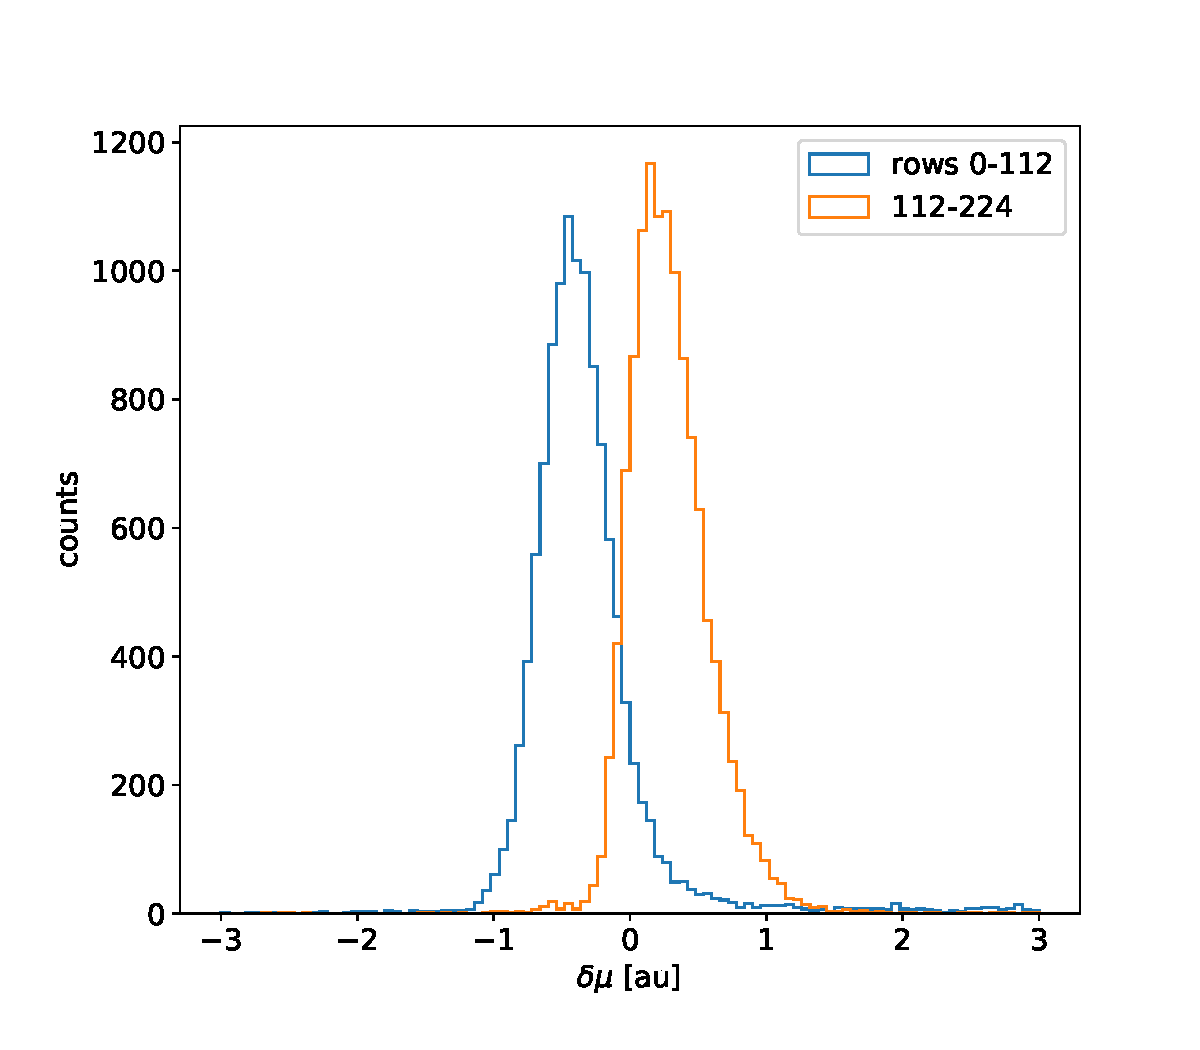
\includegraphics[width=\linewidth]{figures/charaterization/deltam_Fe.pdf}
                \caption{}
                \label{fig:delta_m}
            \end{subfigure}
            \hfill
            \begin{subfigure}[b]{0.49\textwidth}
                \centering
                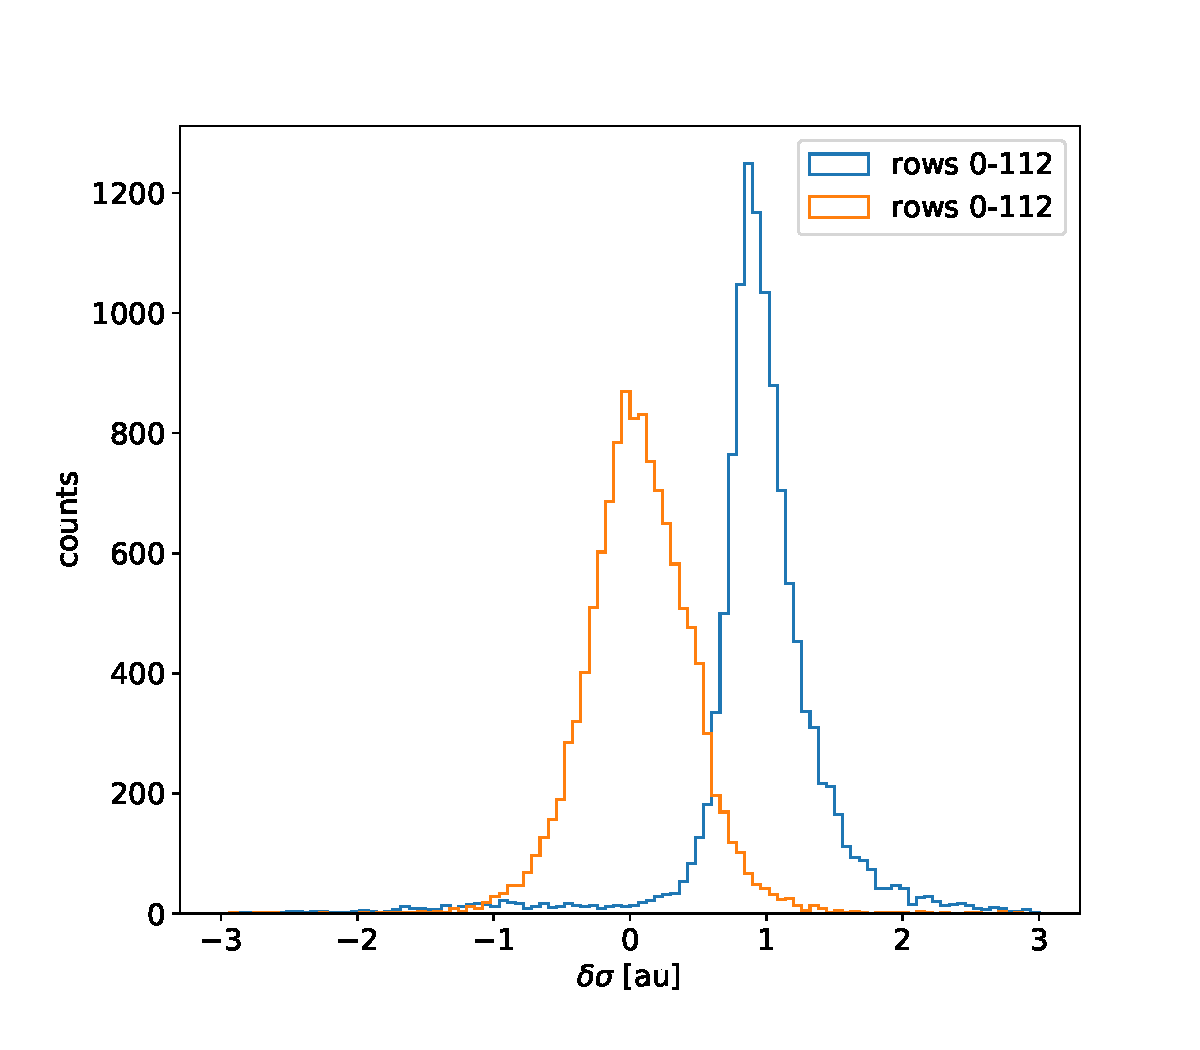
\includegraphics[width=\linewidth]{figures/charaterization/deltas_Fe.pdf}      
                \caption{}
                \label{fig:delta_s}
            \end{subfigure}
            \caption{Difference between the parameters $\mu$ and $\sigma$ obtained with the gaussian fit and those obtained with a gaussian plus a line. When $\mu<$0 the fit with function \ref{eq:gauss} is generally worse (the peak is shifted to the left); when $\sigma<0$, the fit with \ref{eq:gauss_line} is worse (larger sigma). }
            \label{fig:delta_fit}
       \end{figure}        

        The additional linear term in equation \ref{eq:gauss_line} is meant to model the tail due to incomplete charge collection and prevent it from introducing a bias in the fitted peak position.
        For this reason, when I fitted with eq.\ref{eq:gauss_line}, I selected a larger region of the spectrum compared to the fit with eq.\ref{eq:gauss}, for which I used only a small reagion around the peak. The optimal fit range was chosen in both cases through an iterative routine: for the fit with eq.\ref{eq:gauss_line} it starts from an interval including all the ToT above \SI{20}{clock} counts and progressively reduces it by increasing the left boundary; for the fit with eq.\ref{eq:gauss}, it starts from an interval of 5 bins around the expected peak position and reduces the interval of 1 bin at each iteration.
    
        Even if the difference in the peak position between the two fit strategies is not really relevant for the purpose of the calibration, being of the order of 0.8-1.5\% (\ref{fig:delta_fit}), it still introduces a systematic bias towards lower values due to the contribution of the tail. 
        Indeed, we know that the sharp edge on the right must correspond to the case of complete absorption of the photon, so that, in general, the closest to the edge the fitted peak position is, the better the fit is. Besides the peak position, a poor fit tends also to overestimate the peak width. 
        Even looking at the $\chi^2$, the fit function \ref{eq:gauss} seems to be the better choice, except for a set of pixels in the lower part of the matrix, the ones with a FDPW and lower efficiency in pixel corner.

        The resolution of the detector, which is expected to be determined by the statistical fluctuations in the number of charge carries generated in the detector as well as by the ENC, can be compared to the observed Fe55 peak width. Ideally:
        \begin{equation}
            \sigma_{Fe} = \sqrt{ENC^2 \,+ \,F \times N}
        \end{equation}
        Since the number of e/h pairs produced in the sensor is 1616, recalling that the Fano factor F for a silicon detector is 0.115 and that the ENC measured with the injection is \SI{12}{\elementarycharge}$^-$, the $\sigma_{Fe}$ is expected to be $\sim$\SI{18}{\elementarycharge}$^-$. Looking at figure \ref{fig:Fe55_resolution} the resolution achieved with the Fe55 source seems to be much worse. A contribution we have not taken into account but is certainly relevant is the systematic overestimation of the standard deviation of the Fe55 peak: this, as I already explained, is principally due to the high background of incomplete charge collection, which broadens the fitted peak. Although, this effect is not sufficient to justify a such high peak width value. 
        2D maps of the value of the capacity and of the conversion factor found are shown in \ref{fig:capacity_map}. The evident stripe-structure in the matrix shows an evident correlation among the same row; the same structure, which is also visible in the slope map of the calibration of the ToT (fig.\ref{fig:slope_map}), may be related with the structure of the bias lines.\\
        \begin{figure}
            \centering
            \begin{subfigure}[b]{0.49\textwidth}
                \centering
                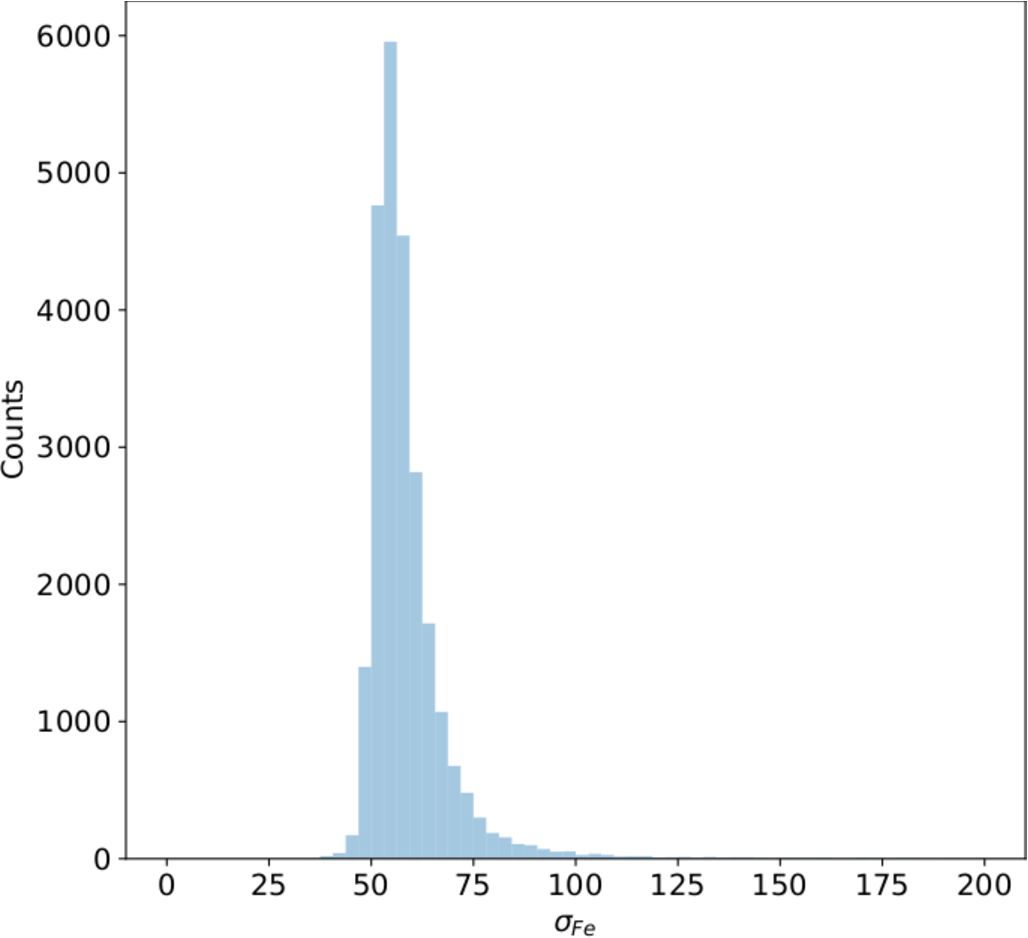
\includegraphics[width=\linewidth]{figures/charaterization/sigma_fe55.pdf} 
                \caption{}
                \label{fig:Fe55_width_hist}
            \end{subfigure}
            \hfill
            \begin{subfigure}[b]{0.49\textwidth}
                \centering
                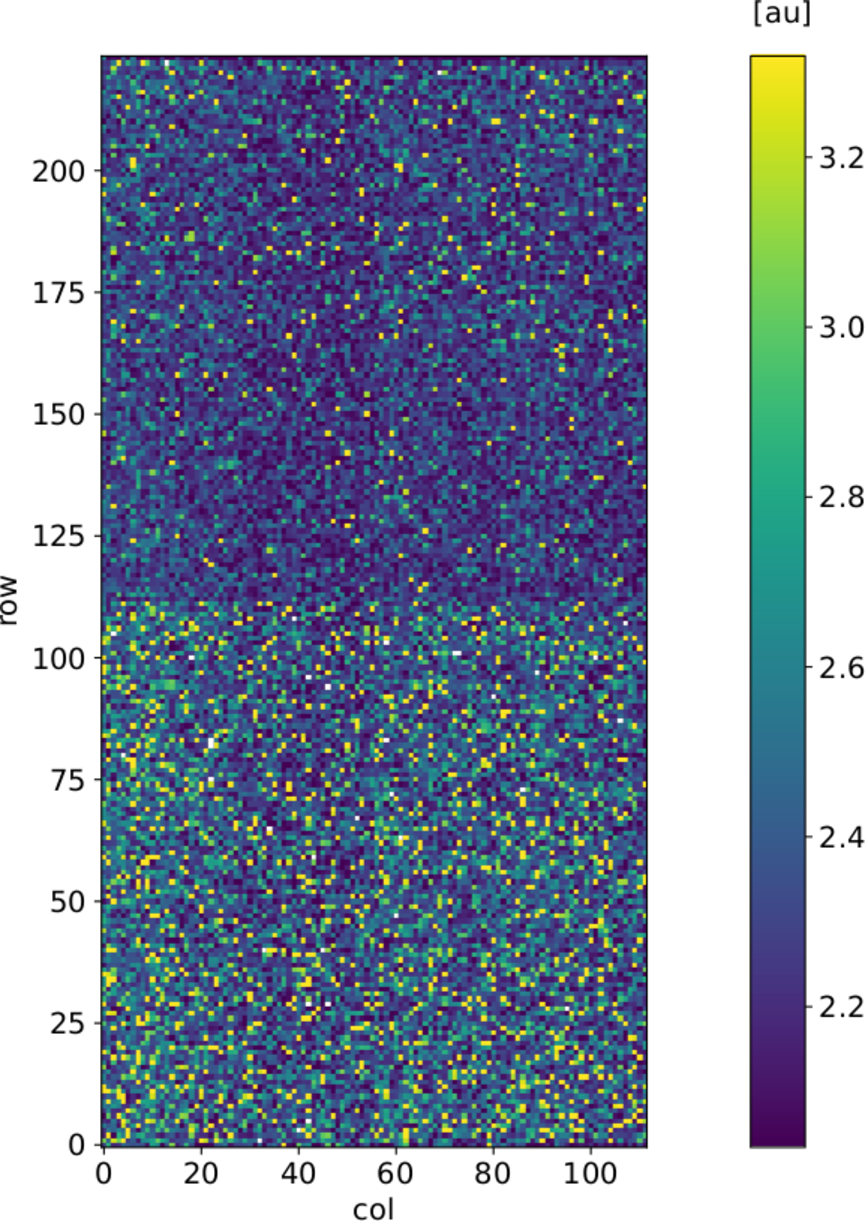
\includegraphics[width=\linewidth]{figures/charaterization/Fe_width_au_map.pdf}   
                \caption{}
                \label{fig:Fe55_width_map}
            \end{subfigure}
            \caption{(a) Histogram and (b) map of the Fe55 width found by the fit with function \ref{eq:gauss} converted in electrons using the calibration. In the map a clear difference between the two parts of the matrix can be be distinguished: in particular, as already stated, the rows with RDPW have a better resolution. It worth noting that the pixels which in the above maps appear disable, here do not show any problem. This prove that they have a problem in the injection circuit but not in the sensor and in the FE.}
            \label{fig:Fe55_resolution}
       \end{figure}  


       \begin{figure}
        \centering
        \begin{subfigure}[b]{0.49\textwidth}
            \centering
            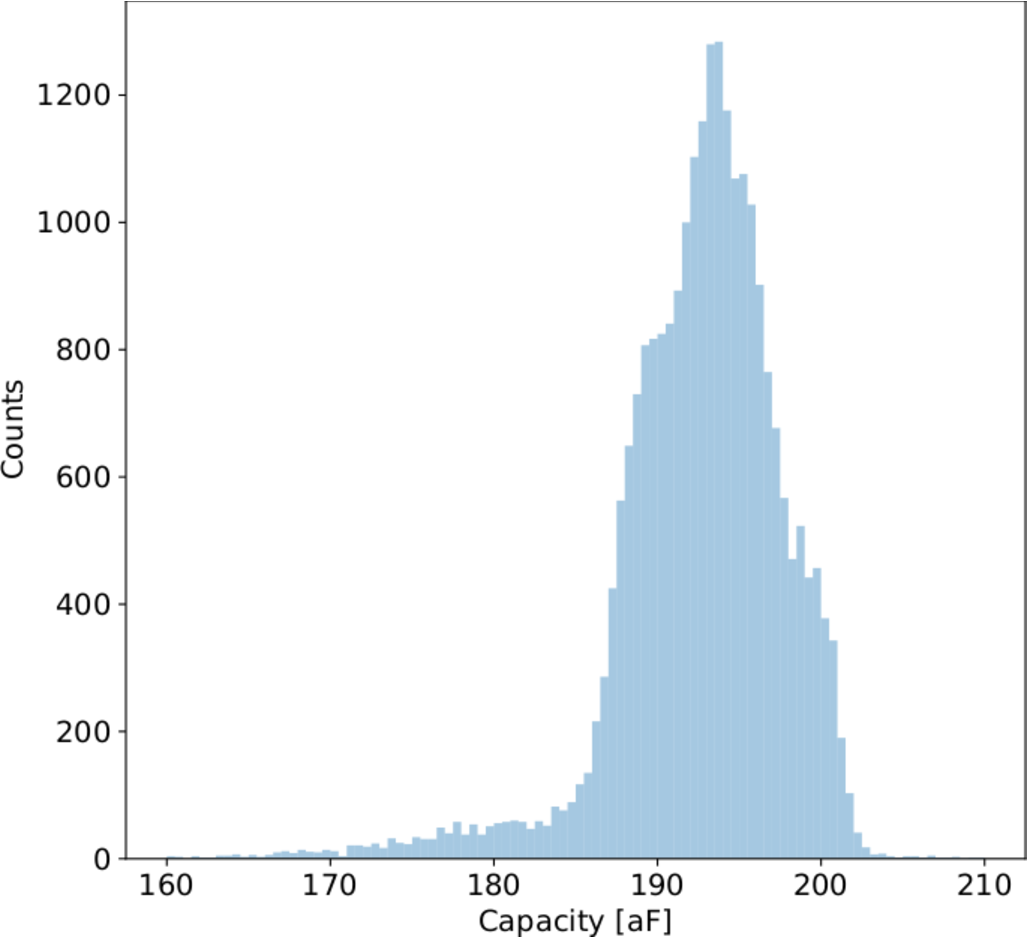
\includegraphics[width=\linewidth]{figures/charaterization/capacity.pdf}
            \caption{}
            \label{fig:}
        \end{subfigure}
        \hfill
        \begin{subfigure}[b]{0.49\textwidth}
            \centering
            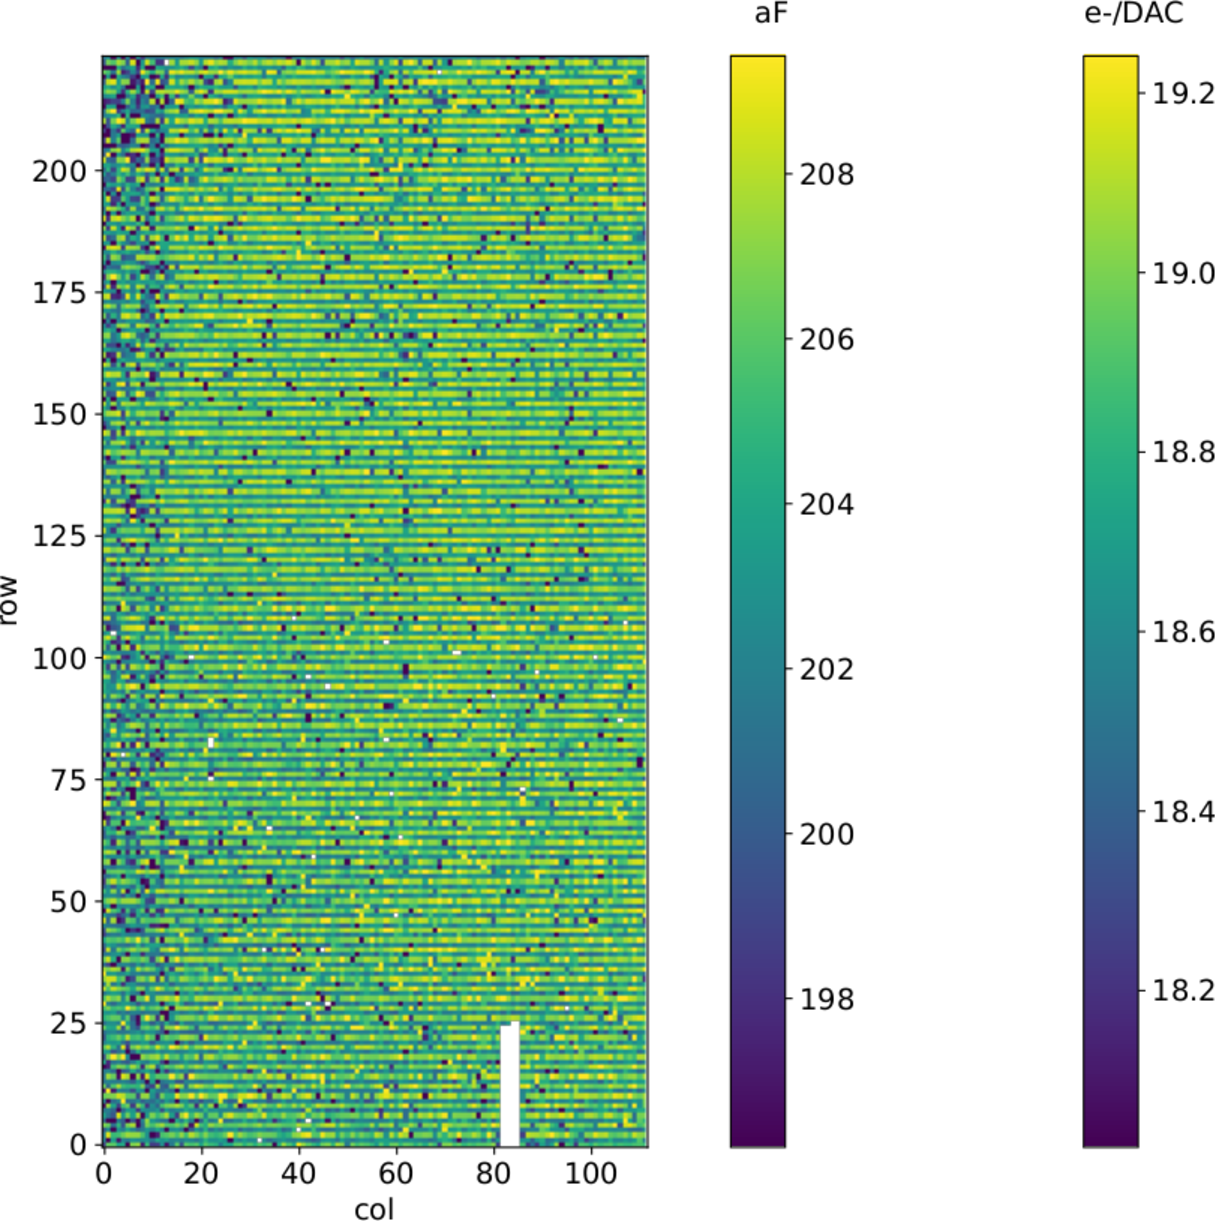
\includegraphics[width=\linewidth]{figures/charaterization/conversion_factor_map.pdf}
            \caption{}
            \label{fig:}
        \end{subfigure}
        \caption{Histogram (a) and map (b) of the calibrated capacity of the injection circuit.}
        \label{fig:capacity_map}
        \end{figure} 

        An attempt of calibrating the HV flavor, which is the most different from the PMOS B flavor, has been performed; however, because of a loss of signal of $\sim$50\% caused by the higher capacitance, we have been unable to identify the Fe55 peak, and then the calibration of the ToT in electrons has been impossible.
        Moreover the HV flavor did not seem to work properly, as we have observed that all pixels sometimes fire one time simultaneously. For these reasons unfortunately a complete characterization of the HV flavor has not been possible: in fact, since it has the most particular FE compared to the other PMOS flavor, a comparing the results would be particularly interesting.
        An example of Fe55 spectrum collected with the HV flavor is shown in figure \ref{fig:HV_fe55}. 
        \begin{figure}[h!]
            \centering
            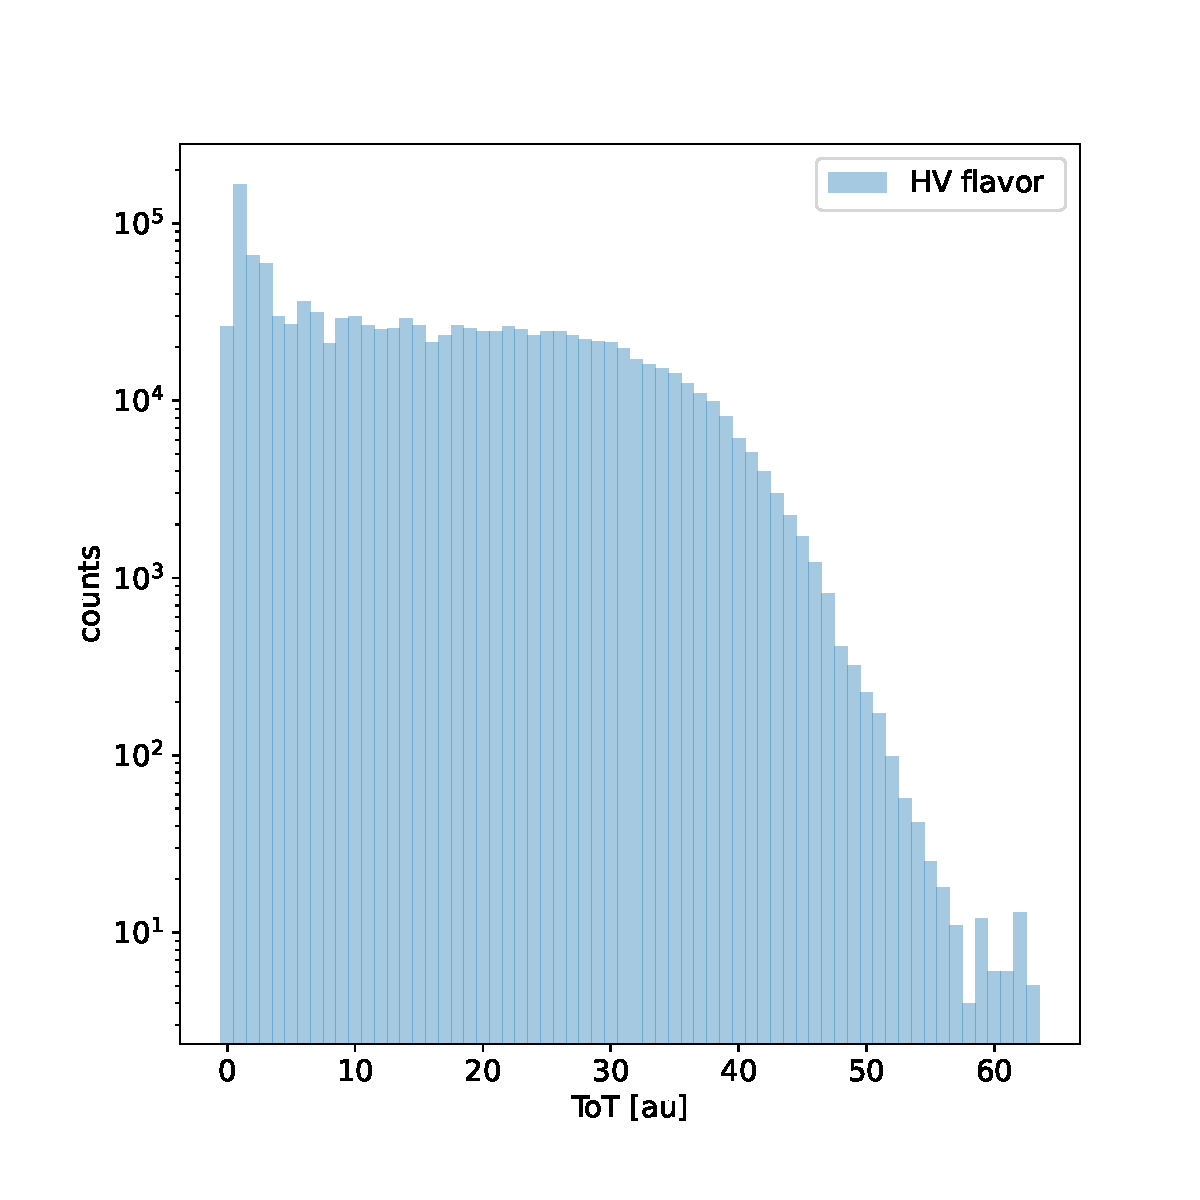
\includegraphics[width=.55\linewidth]{figures/charaterization/Fe55_HV.pdf}
            \caption{Fe55 spectrum with the HV flavor. No peak has been identifyied because of the loss of the signal due to the higher input capacity.}
            \label{fig:HV_fe55}
        \end{figure}  

    \subsection{Changing the bias}\label{chap:characterization_section:bias}
        In order to study the behavior of the sensor as a function of the bias, I performed several injection scans in different sensor bias conditions. 
        The thickness of the depletion region has to be considered an important parameter affecting the signal efficiency, and in particular it affects the charge released by a particle which crosses the sensor, since the signal is proportional to the thickness of the epitaxial layer.
        
        Another important benefit of operating the FE with higher bias is the reduction of the capacitance of the collection diode C$_{in}$, and the corresponding increase of the gain of the first stage of the FE, which goes as $\sim$1/C$_{in}$ (as explained in sec.\ref{sec:ALPIDE-like}). 
        %{With higher gain the ENC is reduced (eq 5.1)   as well as the discriminator threshold and its dispertion that are again reported to equivalent input charge with the usual conversions}\\
        %$THR_{DISC} (e-) = V_{disc} (mV)/gain (mV/e-).$\\
        %$sigma_{THR_DISC} (e-) = V_{rms_disc} (mV) / gain (mV/e-)$
    
        An example of expected change of gain with increased bias is shown in fig.\ref{fig:gain_vs_bias}, that reports the output voltage amplitude and gain for the PMOS and HV flavours for chips characterized by other groups.
        Given that the chip under examination has a gap in the low dose epi-layer (\ref{fig:Monopix1_section_scheme}), we were not able to change independently the bias of the substrate (PSUB) and of the p-well (PWELL), but they must be kept at the same value, differently from other chips of the same submission.
        Lowering the bias, the depletion region is expected to narrow and the efficiency to reduce, especially in the pixel corner, thus raising the threshold and the noise and decreasing the slope as a consequence of the reduction in the gain.
        \begin{figure}[h!]
            \centering
            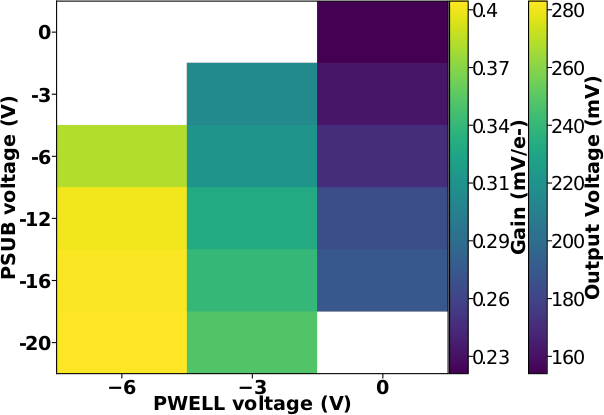
\includegraphics[width=.5\linewidth]{figures/Monopix1/PMOS_gain_bias.png}          
            \caption{Output voltage amplitude and gain with respect to the p-well and p-substrate voltage in the case of the PMOS reset front-end. \red{referenza tesi mustakas} }
            \label{fig:gain_vs_bias}
        \end{figure}  

        In order to test the behavior of the chip when not completely depleted, I have performed an injection scan with PSUB/PWELL bias at \SI{0}{V}, -\SI{3}{V} and -\SI{6}{V} (results in tab.\ref{tab:parameters_vs_bias}); passing from -\SI{6}{V} to a smaller depletion at \SI{0}{V}, the slope of the output signal reduces of $\sim$1/4, which is smaller than the reduction in gain reported in figure \ref{fig:gain_vs_bias}, that is $\sim$1/3. Morover the increase in the threshold and noise at smaller bias is due to the fact that diffusion becomes a competing collection mechaninsm, with all the consequences described in section \ref{sec:MAPS_DMAPS}. 
        Figure \ref{fig:Fe_param_vs_bias} shows the values of the K$_\alpha$ peak position, the normalization of the events above the peak that is the normalization coming from the gaussian fit of the peak, and the rate as a function of the PSUB/PWELL biases. These quantities have been normalized to their value at -\SI{6}{V}, which is then defined as the reference condition. 
        As expected with reduced bias two effects occur: firstly the position of the Fe55 peak moves to lower values due to a lower gain (the reduction of $\sim$1/3 is in agreement with the value measured in \ref{fig:gain_vs_bias}), secondly the number of events in the Fe55 peak and rate both become smaller since the depletion region is reduced.    
        So, what happens is the decrease of both the number of events with full collection (of the \SI{1616}{\elementarycharge}$^-$ from the Fe55 photon) in a single pixel, which contributes to the normalization of the peak, but also the reduction of the events with charge sharing among neighbours pixels. 
    \begin{table}
            \begin{center}
            \begin{tabular}{| c |  c | c | c |}
            \hline
               & -\SI{6}{V} & -\SI{3}{V} & \SI{0}{V}\\
            \hline
            \hline
            Threshold [DAC] & 20 $\pm$ 2 & 21 $\pm$ 2 & 24 $\pm$ 2\\
            Noise [DAC] & 0.61 $\pm$ 0.08 & 0.62 $\pm$ 0.08 & 0.82 $\pm$ 0.1\\
            Slope [au/DAC] & 0.73 $\pm$ 0.03 & 0.71 $\pm$ 0.03  & 0.57 $\pm$ 0.02\\
            Offset [au] & -11 $\pm$ 2 & -11 $\pm$ 2 & -11 $\pm$ 2 \\
            \hline
            \end{tabular}
            \caption{The errors of the values are the standard deviations of the corresponding distributions. To convert DAC values to electrons can be used the conversion factor $\sim$\SI{20}{e-/DAC} (nominal) or $\sim$\SI{18}{e-/DAC} (measured). }
            \label{tab:parameters_vs_bias}
            \end{center}
        \end{table}  
    
        \begin{figure}
            \centering
            \begin{subfigure}[b]{0.49\textwidth}
                \centering
                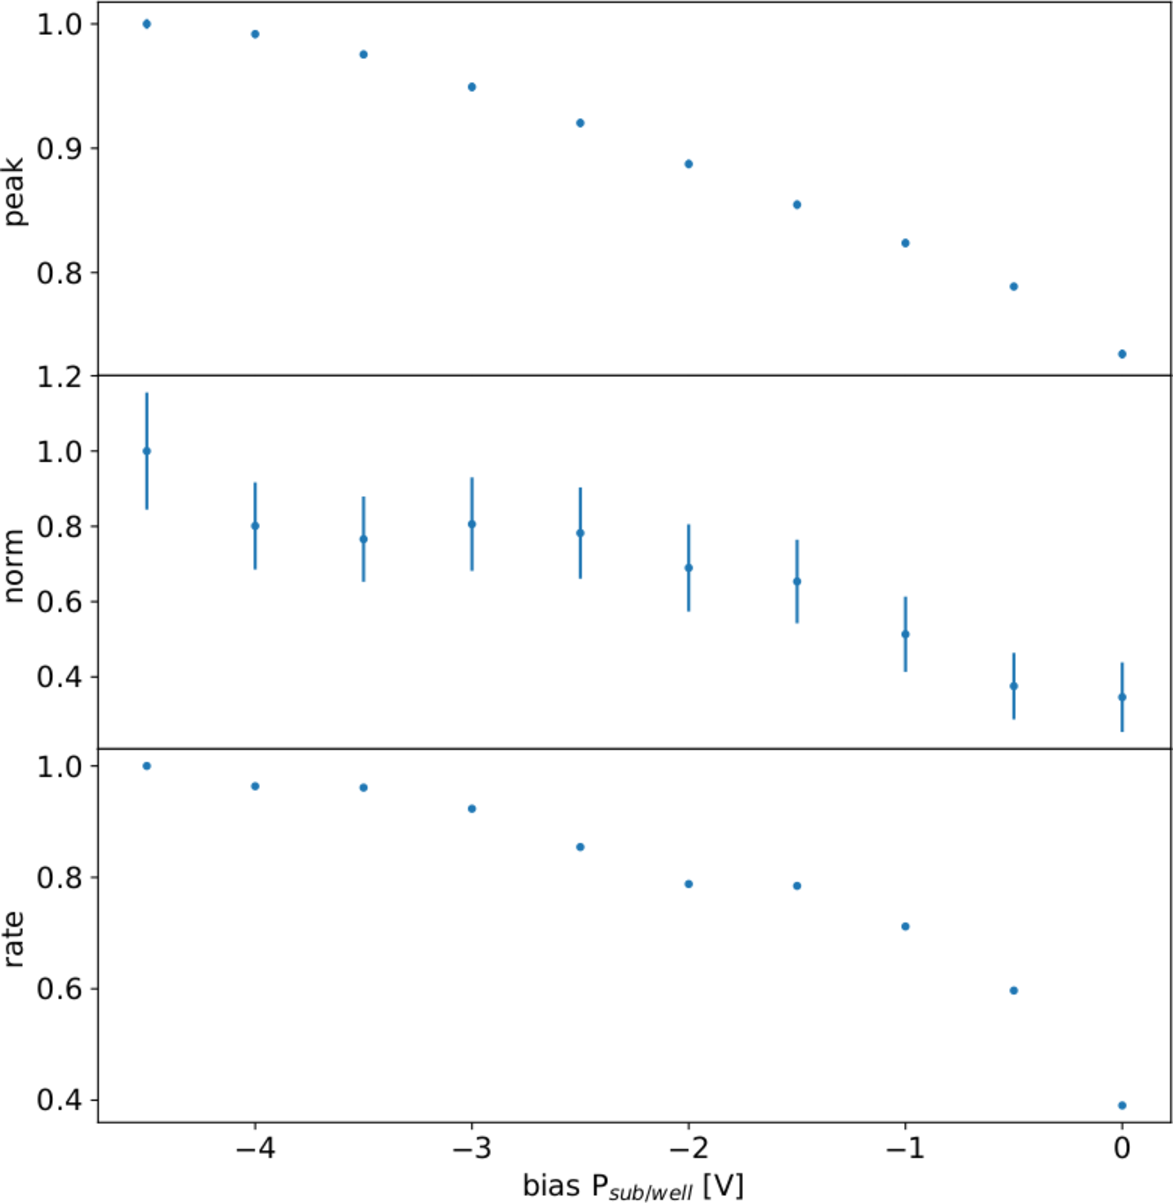
\includegraphics[width=\linewidth]{figures/charaterization/Fe_param_vs_bias.pdf}
                \caption{}
                \label{fig:}
            \end{subfigure}
            \hfill
            \begin{subfigure}[b]{0.49\textwidth}
                \centering
                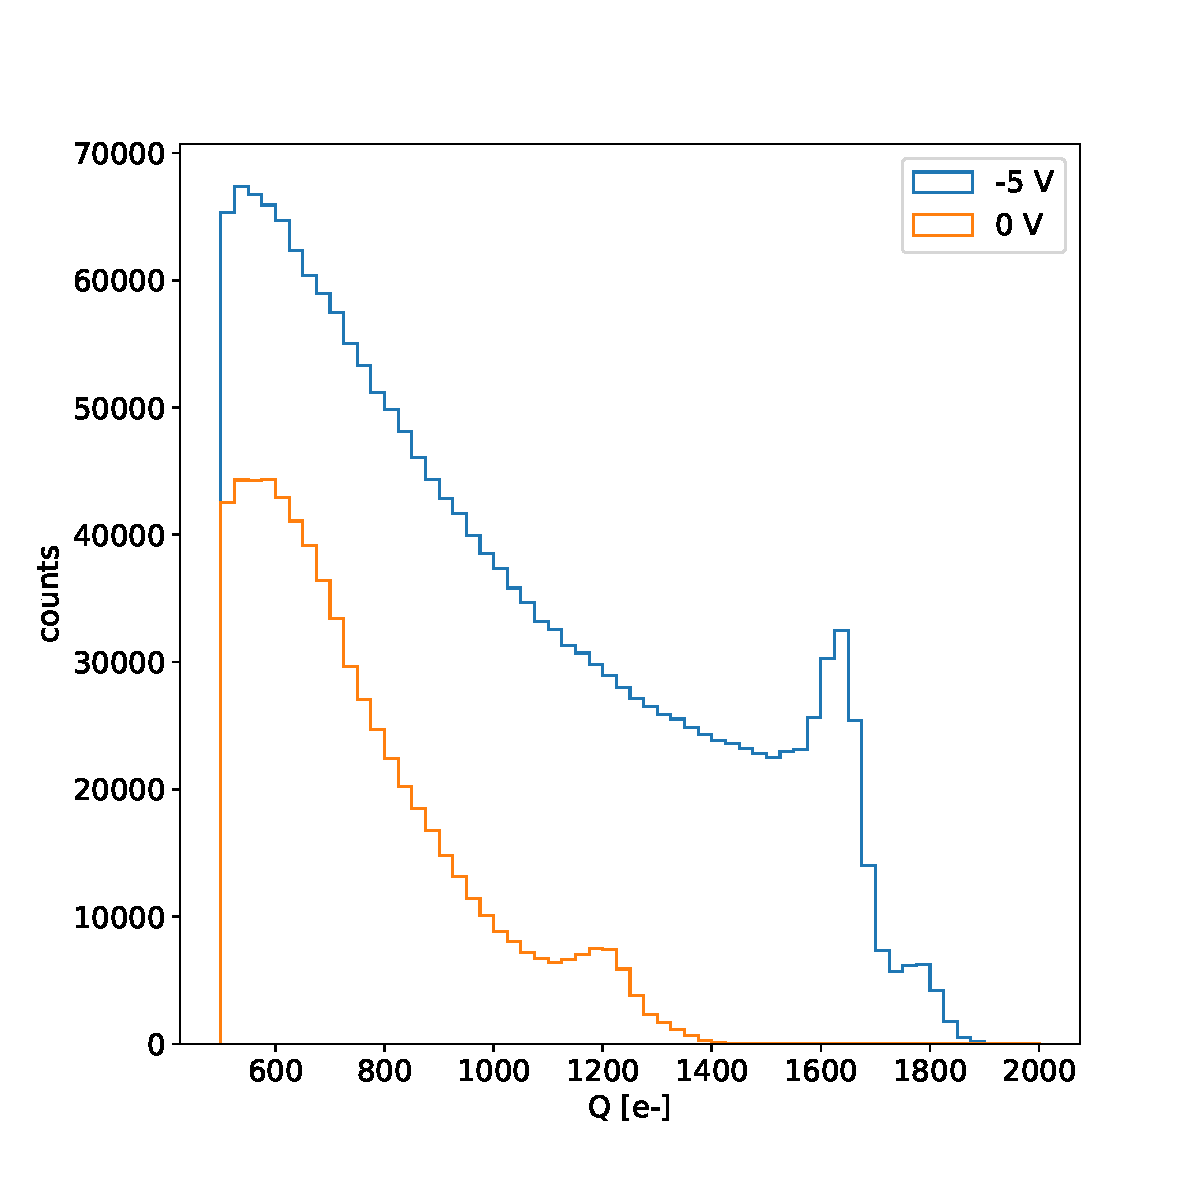
\includegraphics[width=\linewidth]{figures/charaterization/Fe_spectrum_bias.pdf}
                \caption{}
                \label{fig:}
            \end{subfigure}
            \caption{(a) Peak position, peak amplitude and rate as a function of the bias. Since during the collection of the whole data the source has been moved, it is not guaranteed that it has always had a repositioning in the same exactly place, then small the fluctuation of the rate along the decreasing trend are accettable. The peak position and amplitude are estimated by fitting the spectrum with a gaussian in the region around the peak. (b) Fe55 spectrum at different P$_{sub/well}$ bias. The ToT values have been calibrated as explained in section. \ref{sec:cal_ToT}.}
            \label{fig:Fe_param_vs_bias}
            \end{figure}     

    \subsection{Measurements with radioactive sources}\label{sec:sources}
        %python3 -i acquisition_Fe55/find_cluster.py -d acquisition_Fe55/source_PMOSS/noise_acquisitions_6V -> per cluster dimension e spettro del noise
        %python3 -i acquisition_Fe55/hit_map.py -f acquisition_Fe55/source_PMOSS/2022-04-07/2022-04-07_10-10-01_acq.h5 -> per le hit map, comprese qualche hitmap dei cluster
        %python3 -i acquisition_Fe55/Sr90_spectrum.py -d acquisition_Fe55/source_PMOSS/noise_acquisitions_6V/ -> per fare i plot dello stronzio
        In order to completely validate the operation of the whole sensor\footnote{As I will discuss in chapter \ref{sec:Santa_chiara_measurement} these measurements serves also as a reference for the spectrum observed at the test beam}, I have performed several acquisitions with radioactive sources, specifically Fe55 and Sr90Y, which is a $\beta^-$ emettitor with electron endpoint at \SI{2.3}{MeV}, and cosmic rays.
        In particular I used the data collected with Sr90 and cosmic rays, to study charge sharing and events with more than one hit.
        I define \emph{cluster} the ensemble of all the hits with the same timestamp. This is obviously a coarse requirement, but it gave me the opportunity of using a simple and fast clustering algorithm, which is fine when the random coincidence probability is neglibile. 
        Defining R$_1$ and R$_2$ as two any events rate (can be both signal of the same source or one can be a source signal rate and the other the noise rate), and $\tau$ as the dead time of the detector, the random coincidence rate can be found: 
        \begin{equation}
            R_{coinc} = R_1 \, \times\, R_2 \, \times \, \tau
        \end{equation}
        As I am going to prove in the next section, the dead time strictly depends on the occupancy of the matrix, even though we can assume a dead time of $\sim$\SI{1}{\us}, which corresponds to the mean dead time per pixel. However, if in an event a particle hits two different pixels producing a cluster, the total dead time simply doubles. 
        Since the measured rate on the whole matrix of noise, Fe55, Sr90 and cosmic rays are $\sim$\si{Hz}, \SI{3.3}{kHz}, \SI{40}{Hz} and $\sim$\SI{10}{mHz}\footnote{The cosmic rays rate at the sea level is expected to be $\sim$1/cm$^2$/s}, the random coincidence probability are neglibile except the one of two Fe55 events, which is \SI{11}{Hz}.
        
        In figure \ref{fig:cluster_dimension} I report the histograms of the number of pixels in the cluster and of the dimension of clusters, defined in terms of the max and min coordinates on the matrix as:
        \begin{equation}
            d = \sqrt{(y_{max}-y_{min})^2 + (x_{max}-x_{min})^2}
        \end{equation}\label{eq:cluster_dimension}
        Looking at the shape of the histogram of the dimension, generally the Sr90 and the cosmic rays produce bigger clusters and hit a higher number of pixels, a trend that can be explained considering that the Fe55 photoelectron is less energetic than the Sr90 electron and cosmic rays. 
        \begin{figure}
            \centering
            \begin{subfigure}[b]{0.49\textwidth}
                \centering
                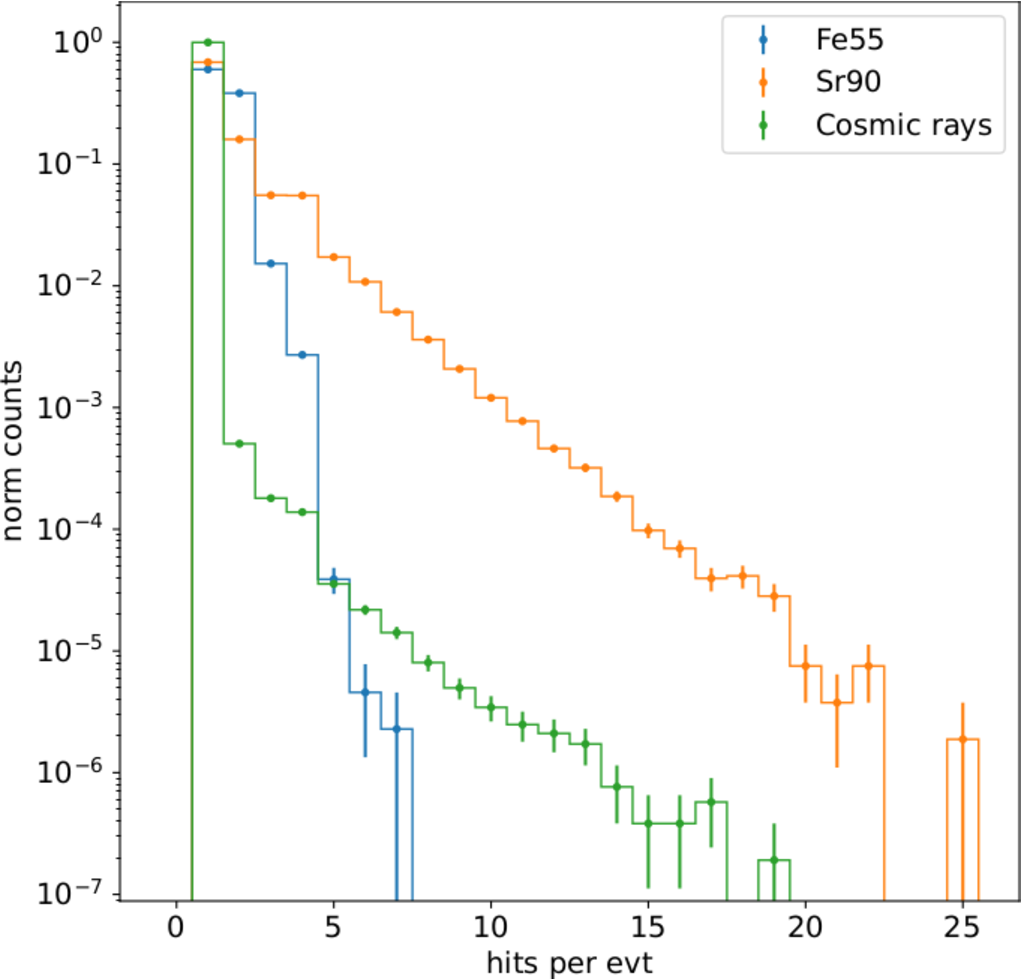
\includegraphics[width=\linewidth]{figures/charaterization/hits_per_evt.pdf}
                \caption{}
                \label{fighits_per_cluster:}
            \end{subfigure}
            \hfill
            \begin{subfigure}[b]{0.49\textwidth}
                \centering
                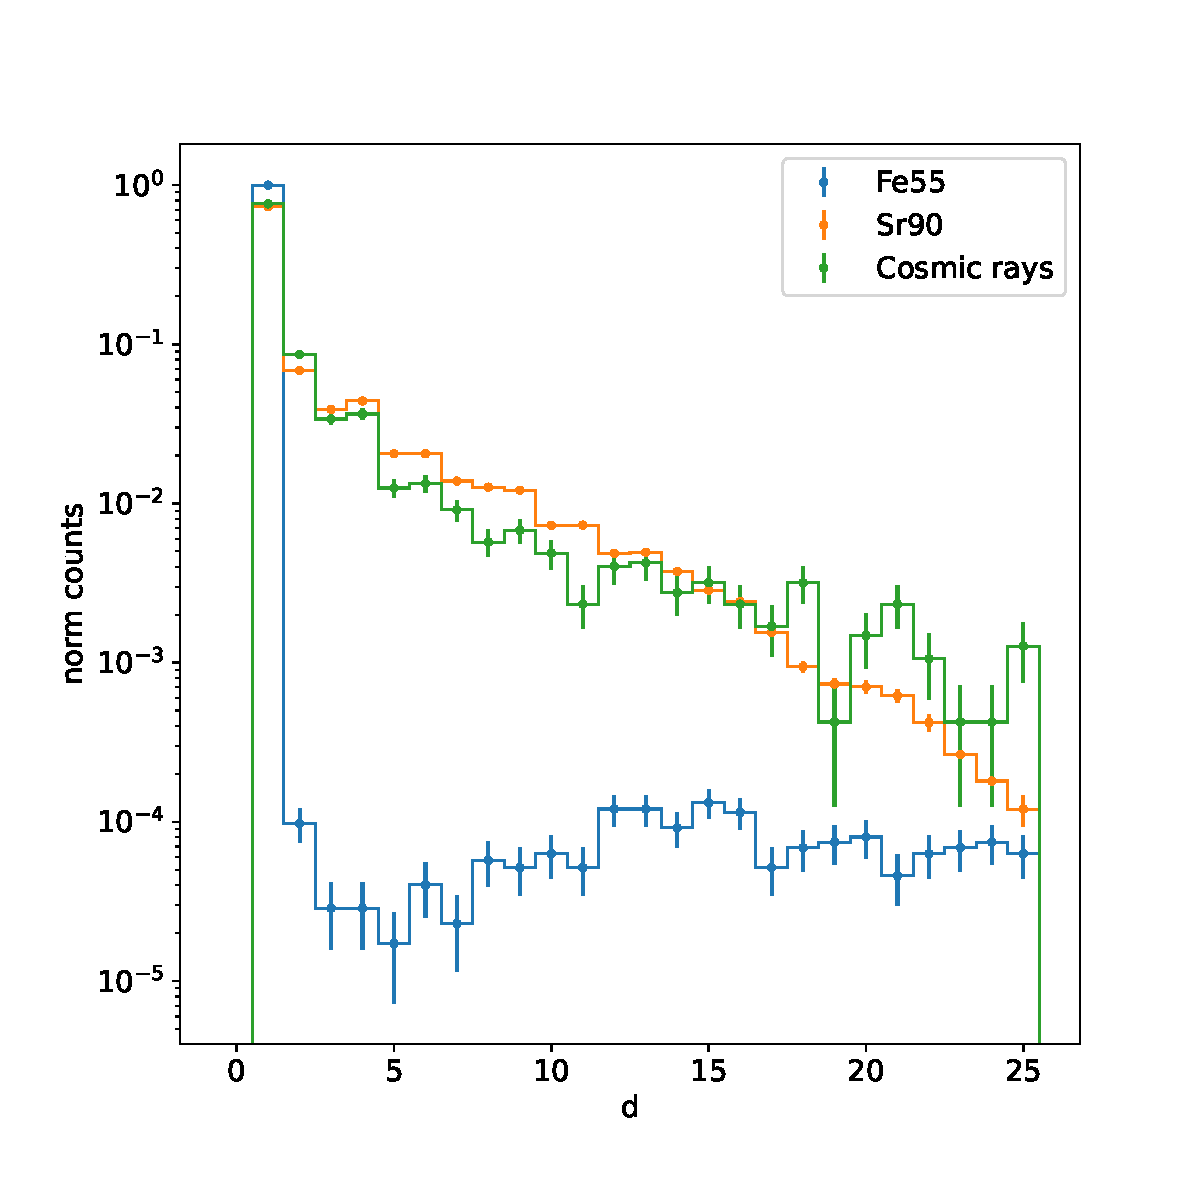
\includegraphics[width=\linewidth]{figures/charaterization/cluster_dimension.pdf}
                \caption{}
                \label{fig:cluster_dimension}
            \end{subfigure}
            \caption{(a) Distribution of the number of hits per event with different sources. (b) Dimension of cluster defined as eq.\ref{eq:cluster_dimension}. Compared with the Sr90 and the cosmic rays, the Fe55 d distribution is characterized by a clear discontinuity around d=5. The very thin peak at 0 corresponds to the effective clusters, while the long tail at bigger d is principally made of random coincidences distant on the matrix.}
            \label{fig:cluster_dimension}
            \end{figure}  
        A sample of hitmap of events produced by the three different sources is shown in figures \ref{fig:hit_map_cosmic_rays}, \ref{fig:hit_map_Sr90} and \ref{fig:hit_map_Fr550}. 
        \begin{figure}[h!]
            \centering
            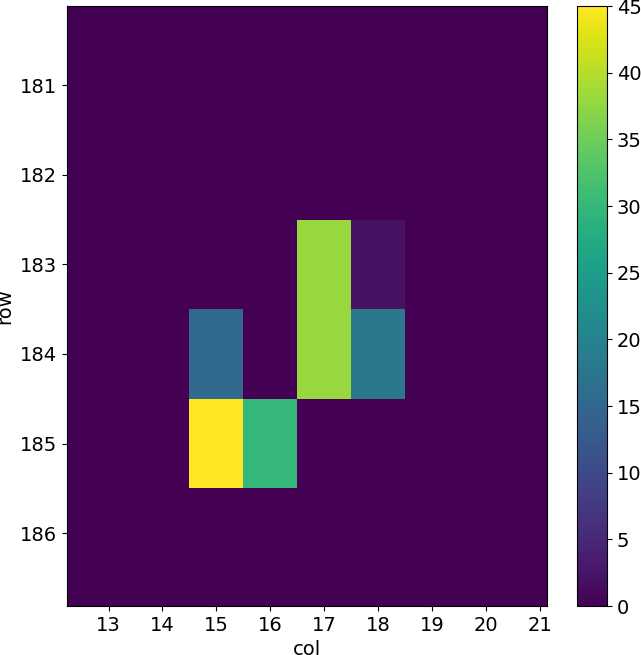
\includegraphics[width=.24\linewidth]{figures/charaterization/evts/cosmic_rays/7a.png}
            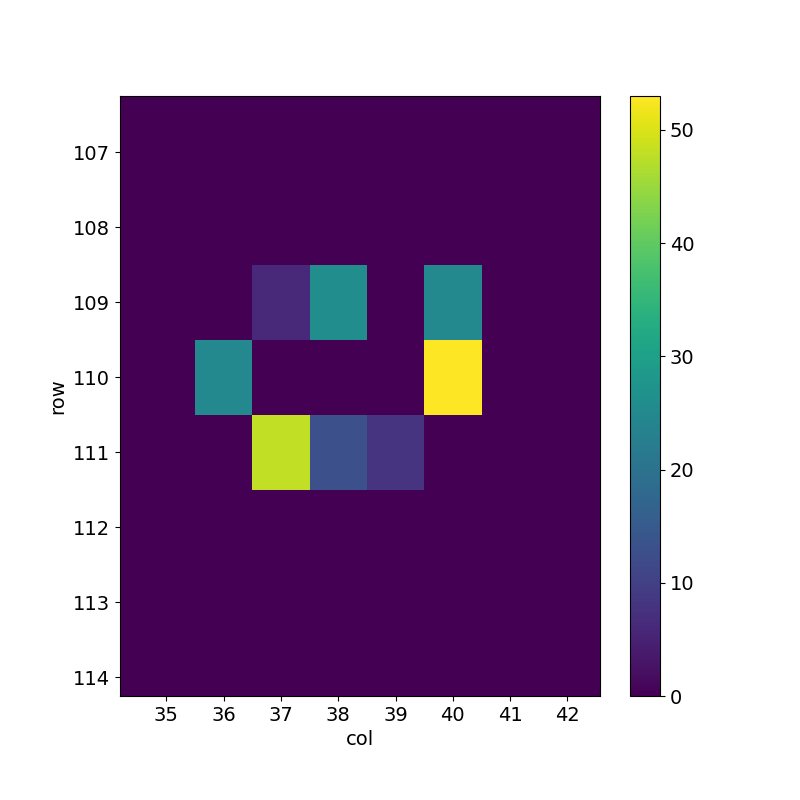
\includegraphics[width=.24\linewidth]{figures/charaterization/evts/cosmic_rays/8a.png}
            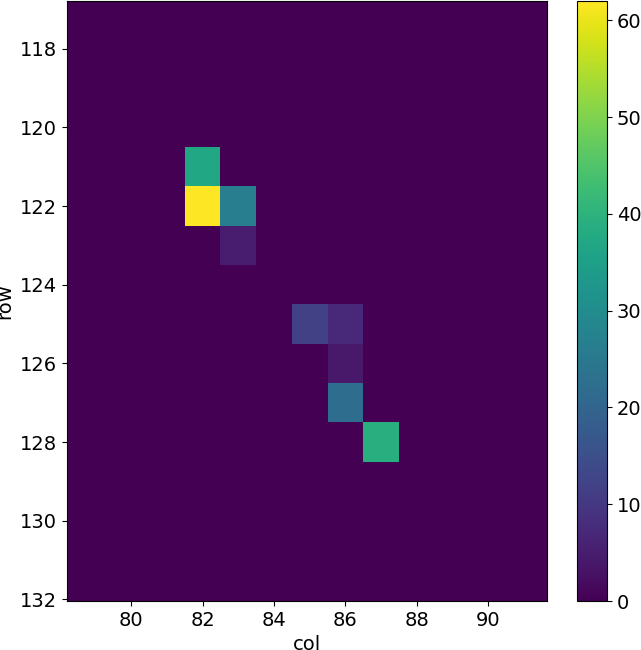
\includegraphics[width=.24\linewidth]{figures/charaterization/evts/cosmic_rays/9c.png} 
            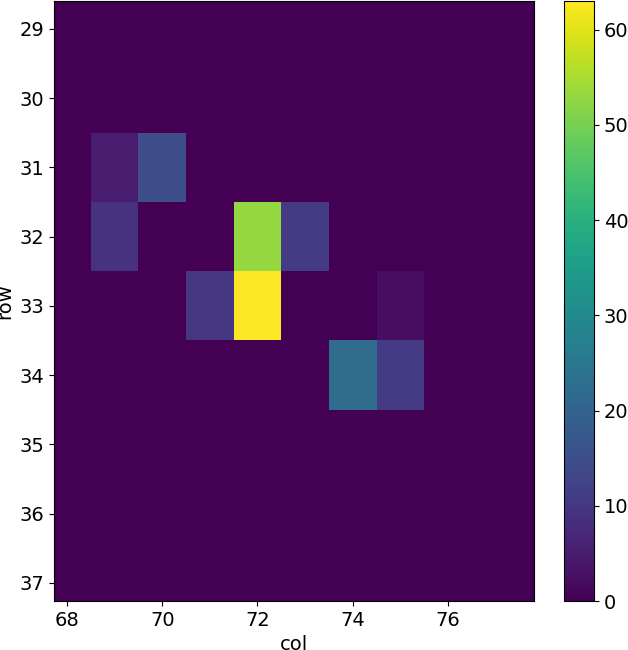
\includegraphics[width=.24\linewidth]{figures/charaterization/evts/cosmic_rays/10a.png}\\
            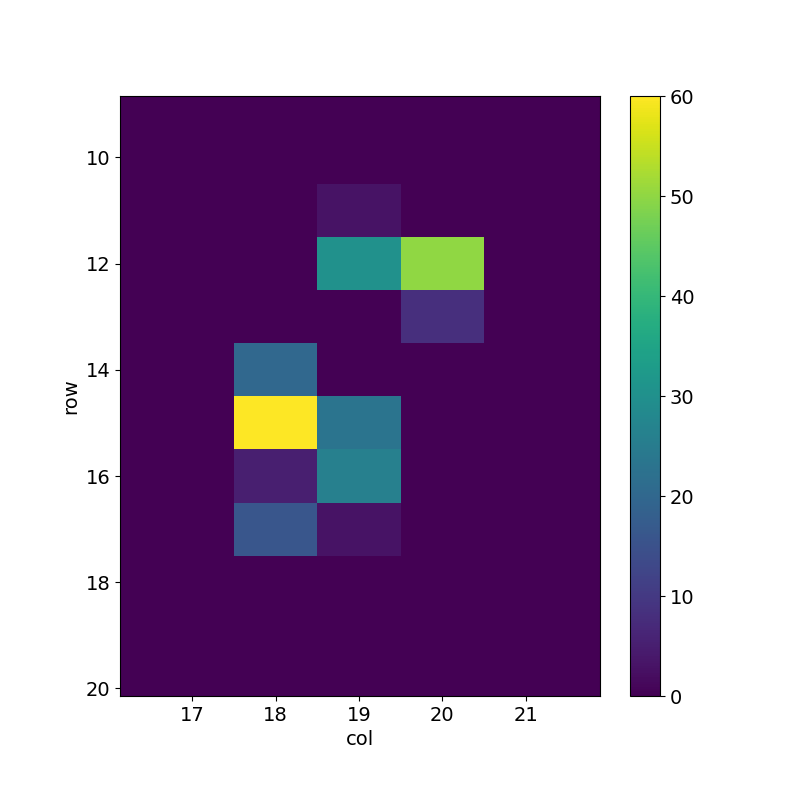
\includegraphics[width=.24\linewidth]{figures/charaterization/evts/cosmic_rays/11a.png}
            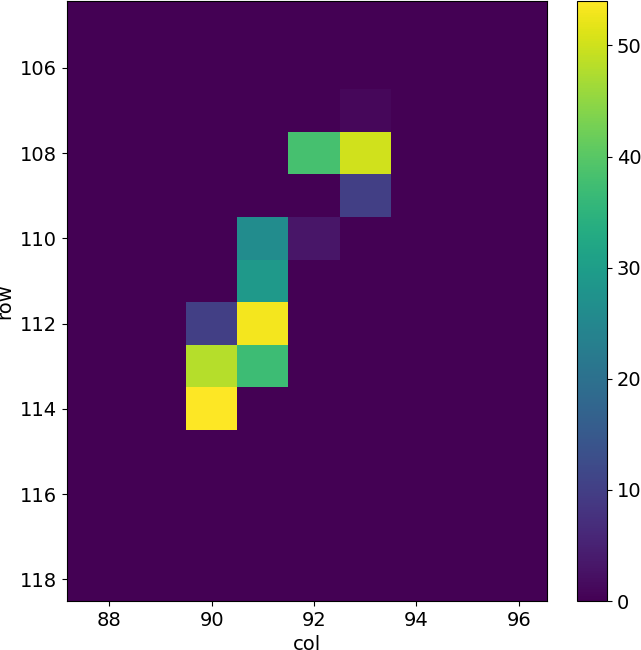
\includegraphics[width=.24\linewidth]{figures/charaterization/evts/cosmic_rays/12.png}
            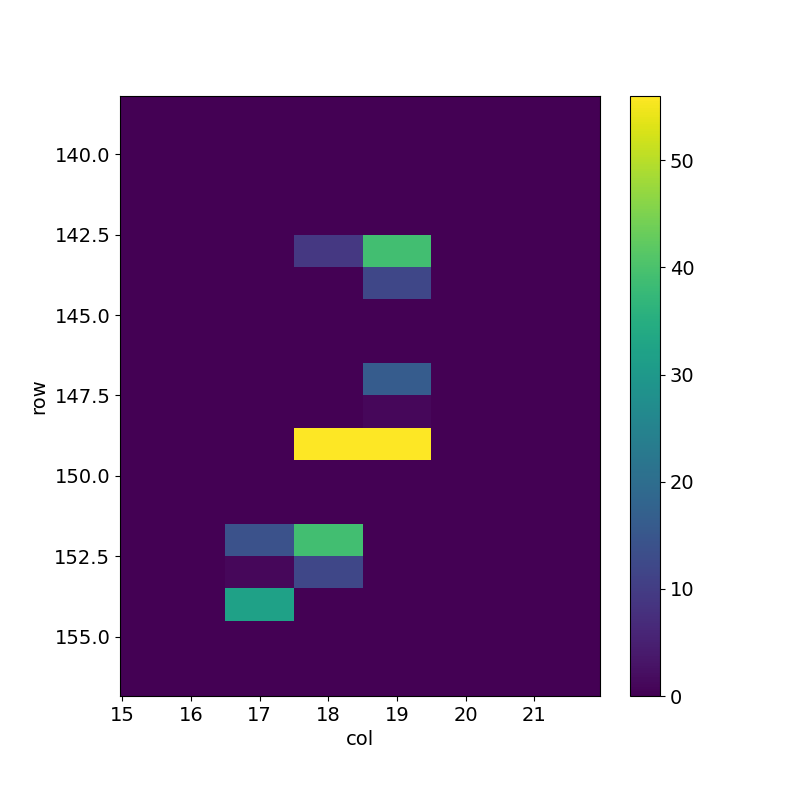
\includegraphics[width=.24\linewidth]{figures/charaterization/evts/cosmic_rays/12b.png}               
            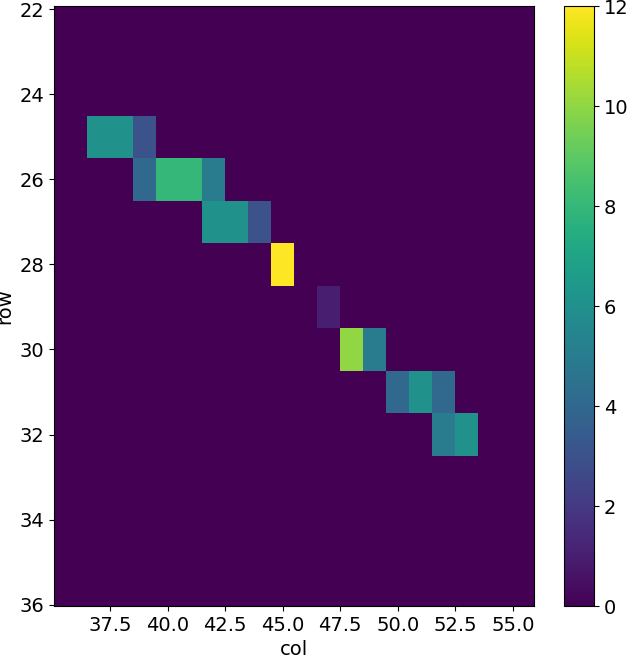
\includegraphics[width=.24\linewidth]{figures/charaterization/evts/cosmic_rays/19a.png}
            \caption{2D histograms of the ToT in different events in an aquisition of cosmic rays.}
            \label{fig:hit_map_cosmic_rays}
        \end{figure} 
        \begin{figure}[h!]
            \centering
            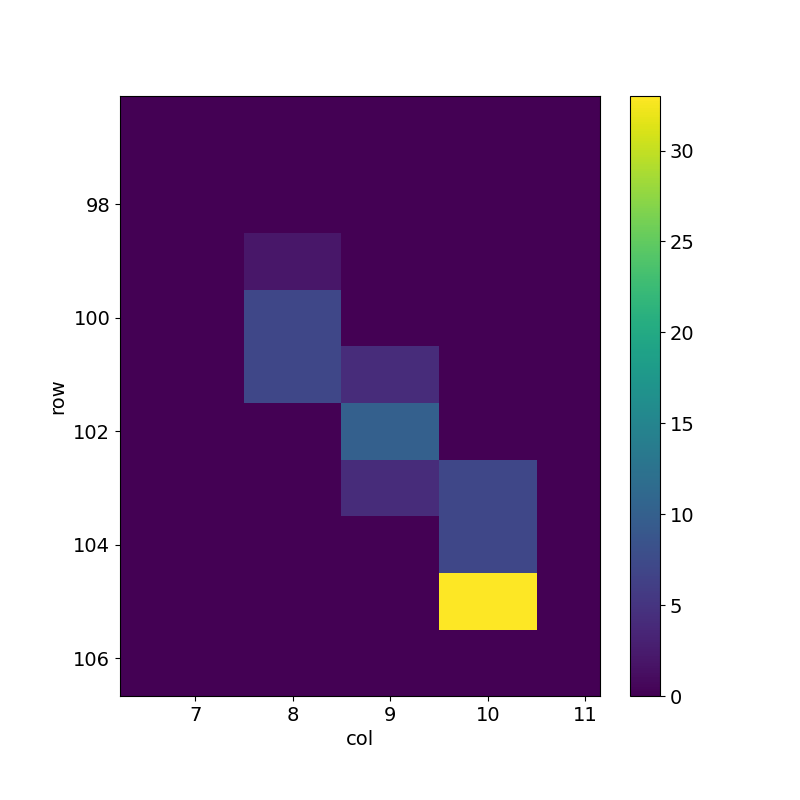
\includegraphics[width=.24\linewidth]{figures/charaterization/evts/Sr90/9b.png}
            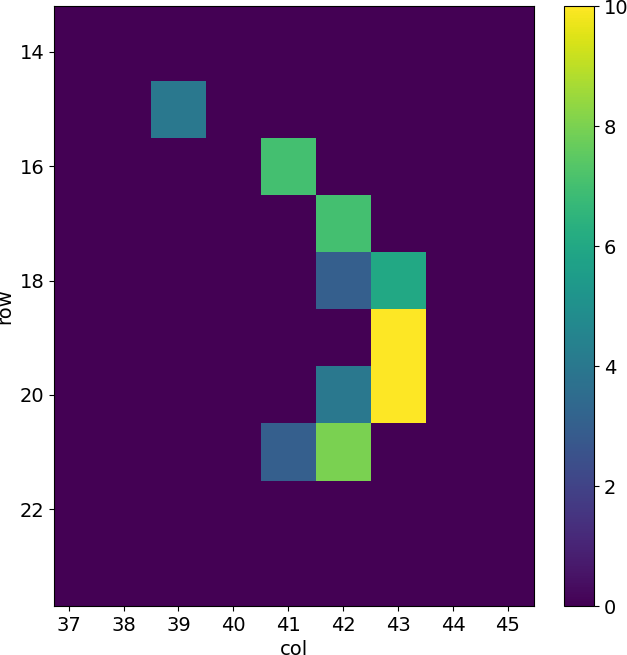
\includegraphics[width=.24\linewidth]{figures/charaterization/evts/Sr90/10b.png}
            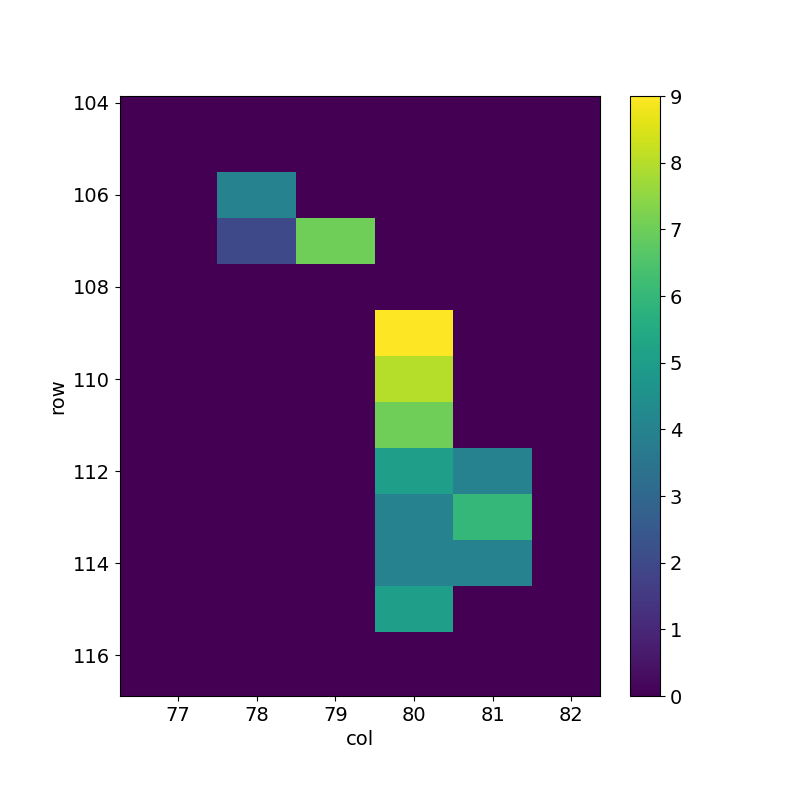
\includegraphics[width=.24\linewidth]{figures/charaterization/evts/Sr90/13a.png}
            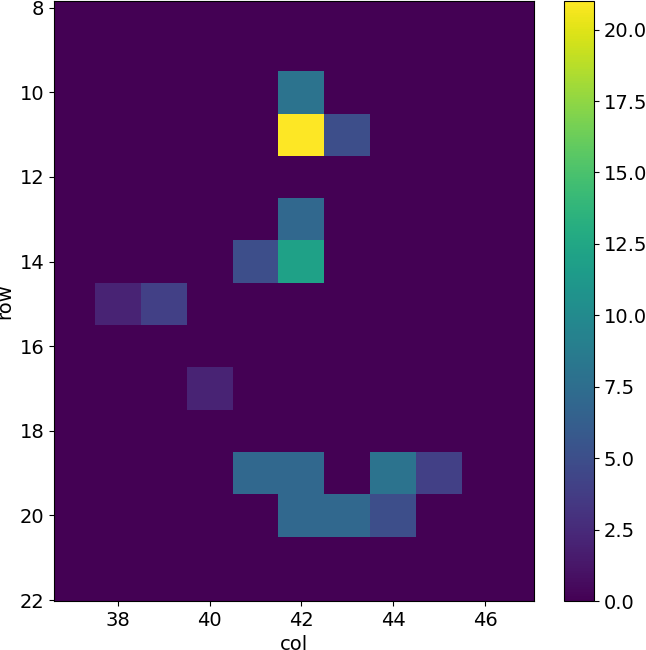
\includegraphics[width=.24\linewidth]{figures/charaterization/evts/Sr90/16a.png}
            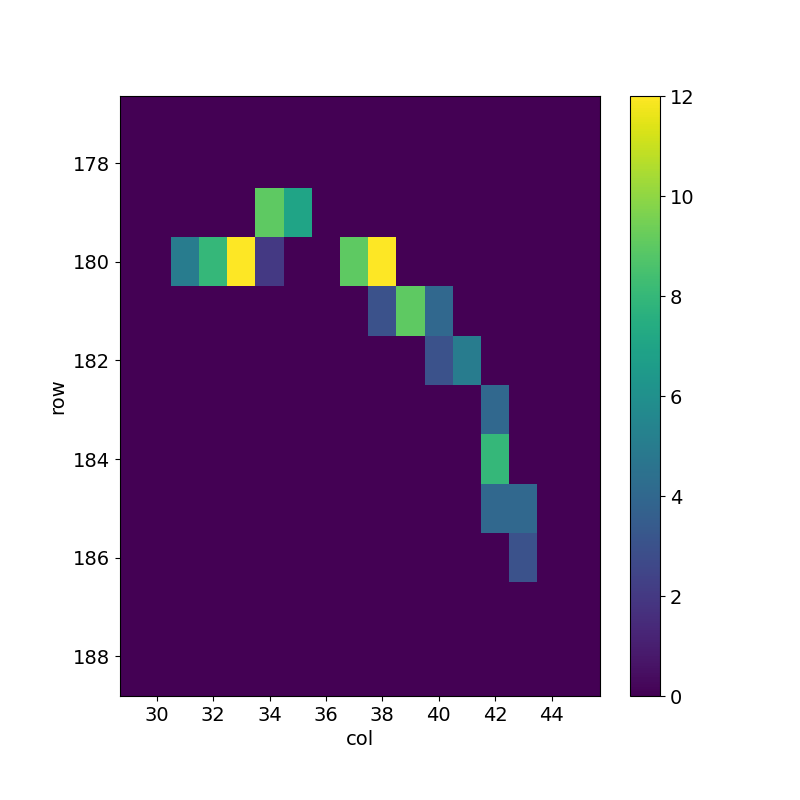
\includegraphics[width=.24\linewidth]{figures/charaterization/evts/Sr90/18b.png}
            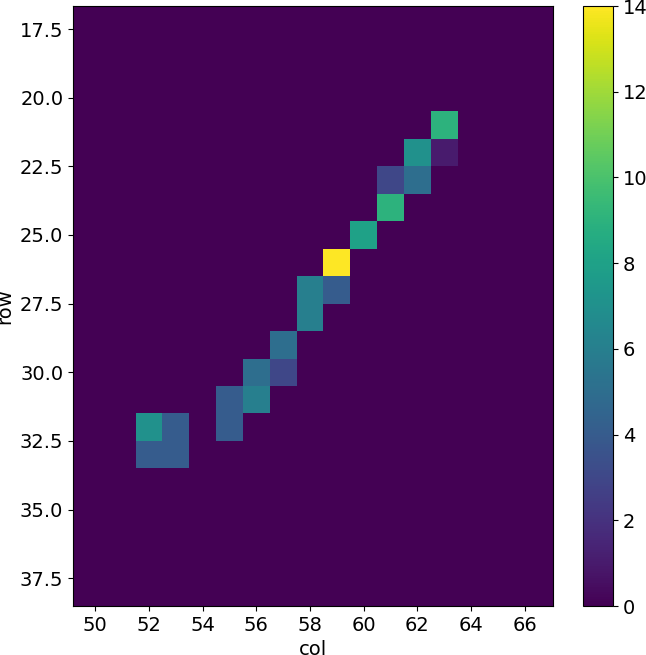
\includegraphics[width=.24\linewidth]{figures/charaterization/evts/Sr90/21a.png}
            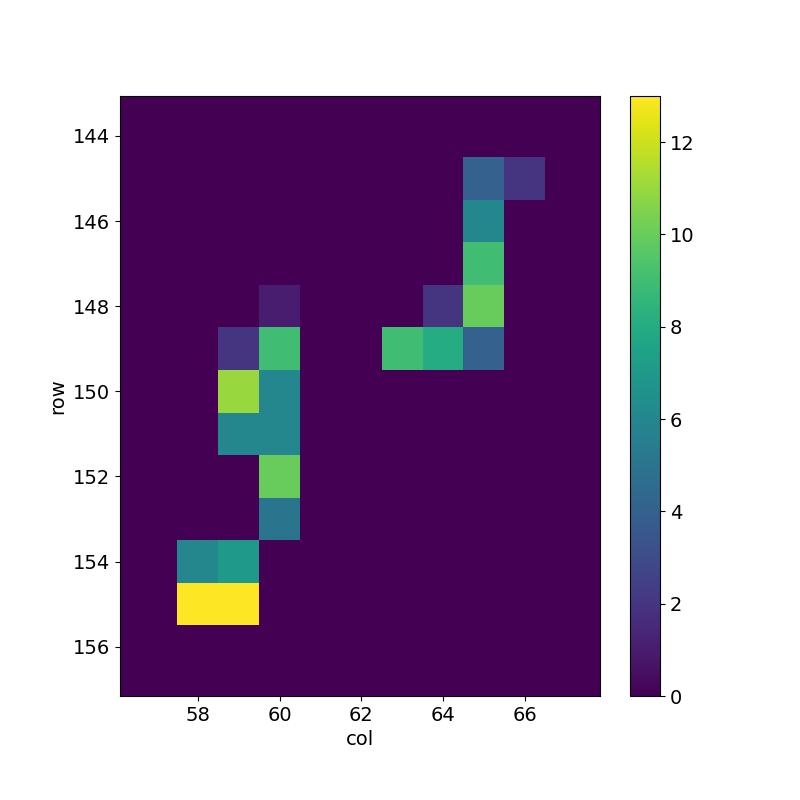
\includegraphics[width=.24\linewidth]{figures/charaterization/evts/Sr90/22a.png}
            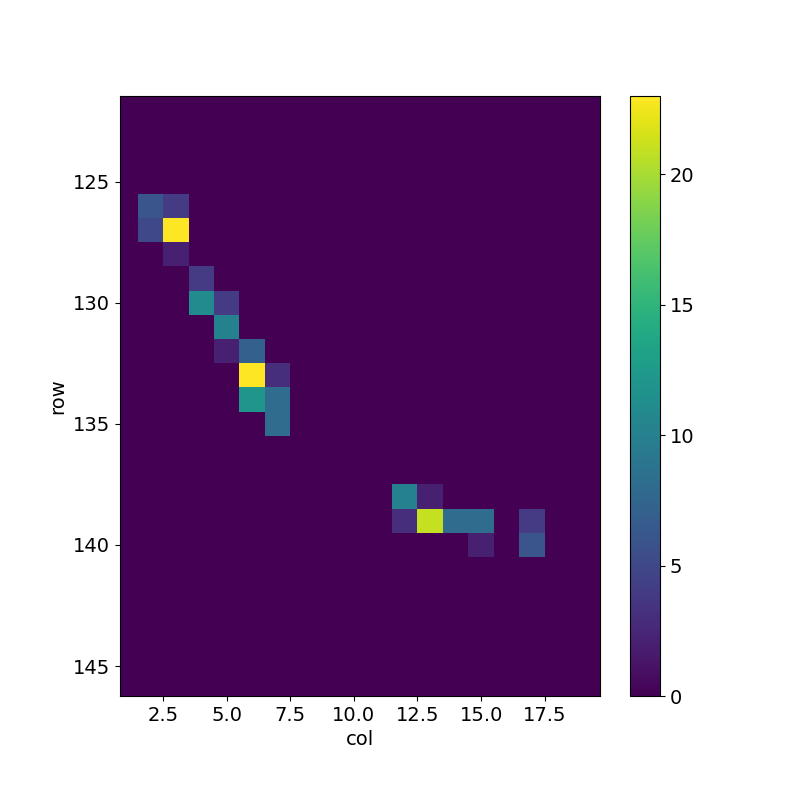
\includegraphics[width=.24\linewidth]{figures/charaterization/evts/Sr90/25a.png}               
            \caption{2D histograms of the ToT in different events in an aquisition of Sr90.}
            \label{fig:hit_map_Sr90}
        \end{figure}         
        \begin{figure}[h!]
            \centering
            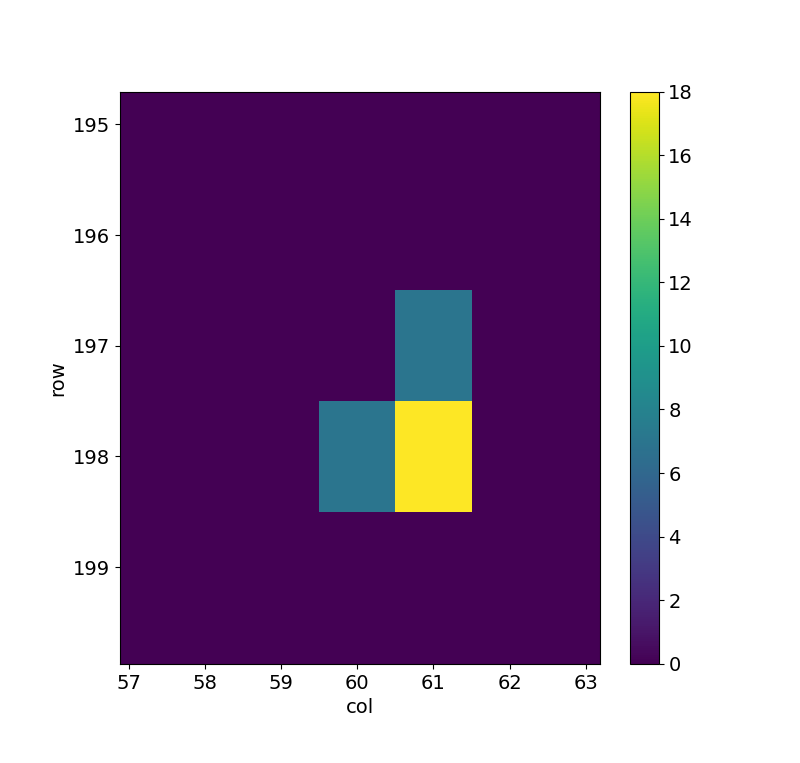
\includegraphics[width=.24\linewidth]{figures/charaterization/evts/Fe55/3a.png}
            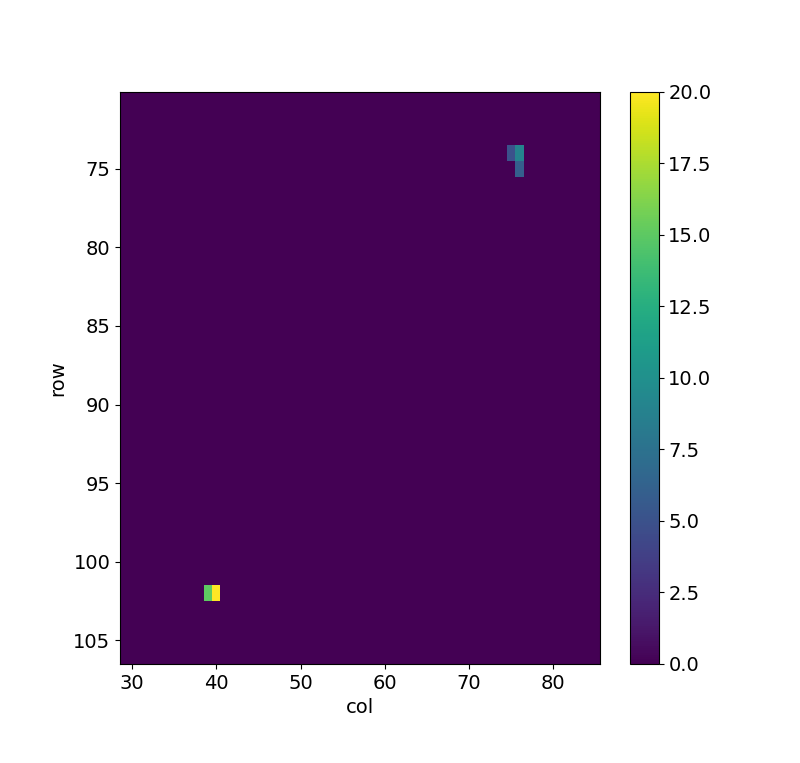
\includegraphics[width=.24\linewidth]{figures/charaterization/evts/Fe55/5a.png}
            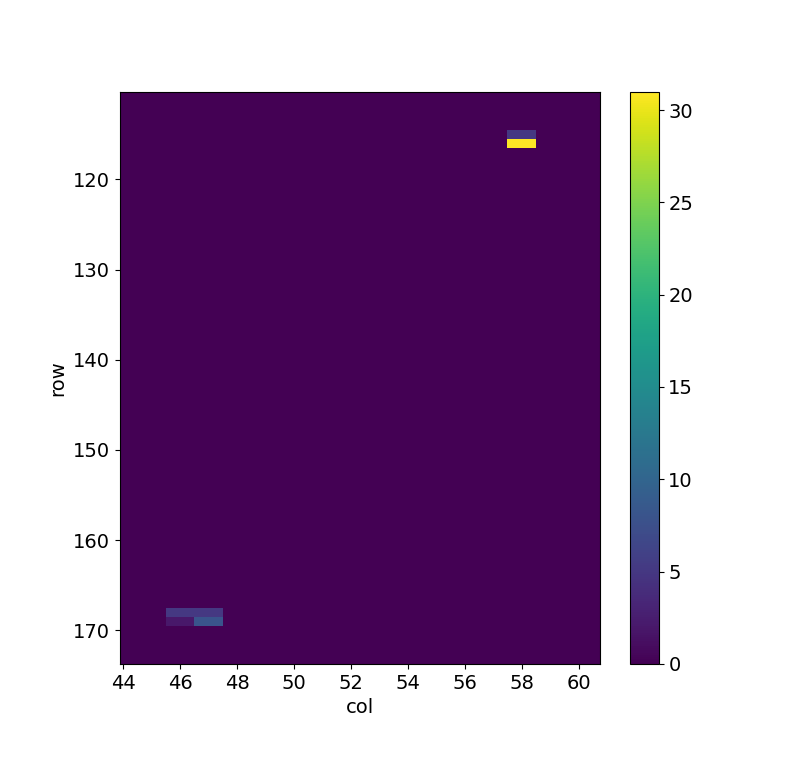
\includegraphics[width=.24\linewidth]{figures/charaterization/evts/Fe55/6a.png}
            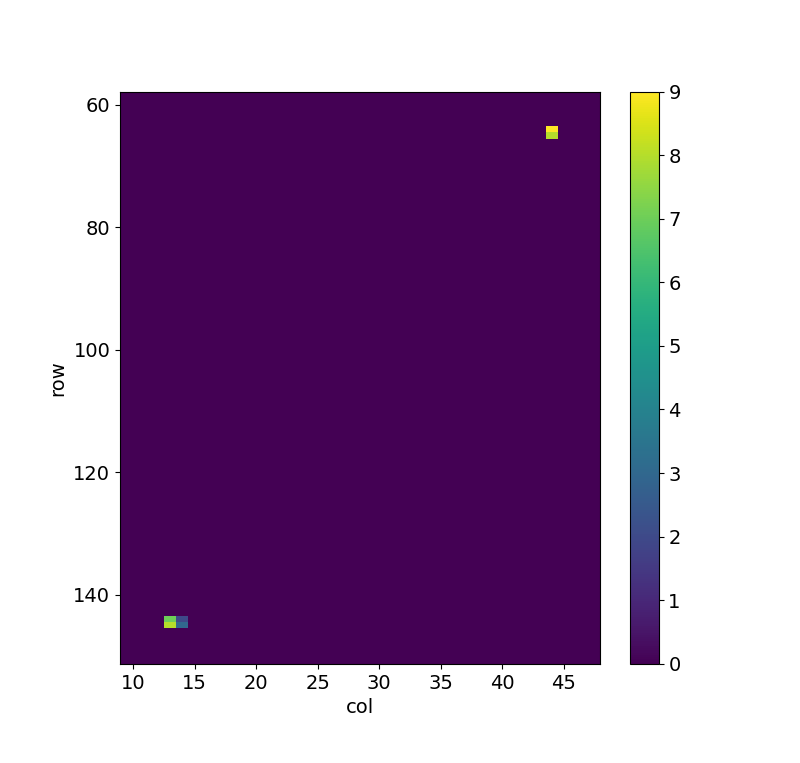
\includegraphics[width=.24\linewidth]{figures/charaterization/evts/Fe55/6b.png}
            \caption{2D histograms of the ToT in different events in an aquisition of Fe55}
            \label{fig:hit_map_Fr550}
        \end{figure} 
        In figures \ref{fig:spectrum_cosmic_rays}, \ref{fig:spectrum_Sr90}, \ref{fig:spectrum_Fe55} are shown the distributions per different cluster dimension events, of the charge collected by a single pixel (figures on the left) and the charge collected by summing the charge collected by the pixels within the cluster (figures on the right). 
        Since the noise rate is comparable with the cosmic rays and Sr90 ones, I have removed the single pixel events which are separately shown in figure \ref{fig:single_pixel_cluster}; although we cannot identify and select only the noise events, these distributions, and especially the cosmic rays one, are expected to be mostly populated by noise events.  
        The distributions have a peak around the threshold, which is compatible with the fact that the noise events typically have a low ToT. 
    
        Looking at the spectra of Sr90 instead (fig:\ref{fig:spectrum_Sr90}), the maximum of the distribution of the cluster charge seems to follow a linear dependence on the number of pixels hit (tab.\ref{tab:charge_cluster}); this can be accepted as a first approximation considering that the pitch (\SI{36}{\um} and \SI{40}{\um}) depends on the direction, and the epitaxial layer thickness (25-30\si{\um}) are comparable. 
        However a more accurate model which takes into account the impact angle of the particle and charge sharing among neighbours pixels should be developed for a more precise comparison.
        \begin{figure}
            \centering
            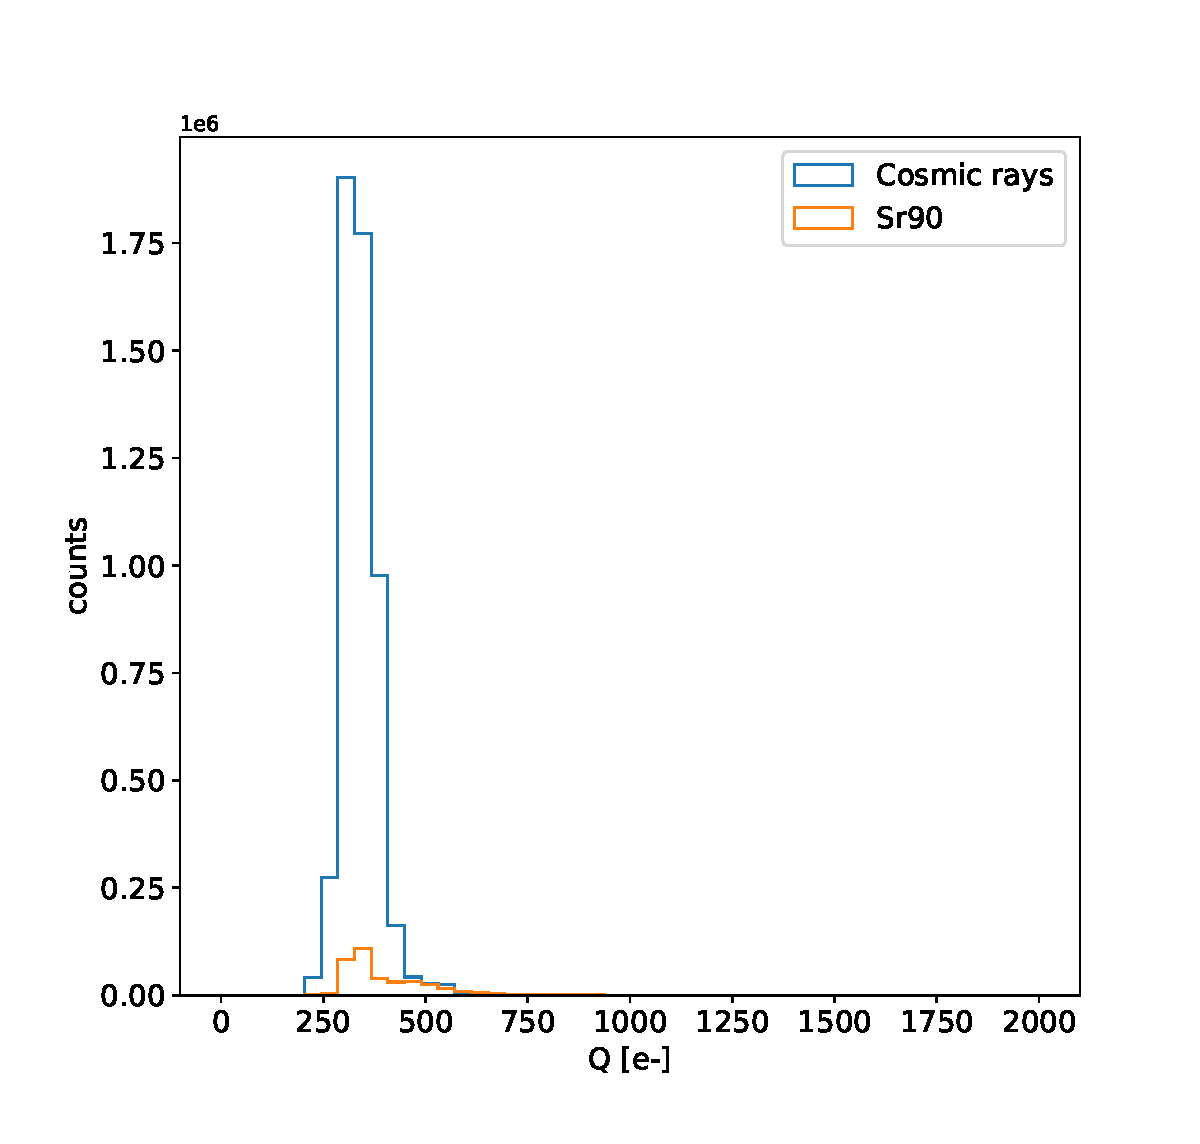
\includegraphics[width=.6\linewidth]{figures/charaterization/background.pdf}
            \caption{Histograms of the charge released in the pixels in events in which only a single pixel turns on.}
            \label{fig:single_pixel_cluster}
        \end{figure}         
        %\red{The charge per length covered $Q/l$ released by a particle which crosses more pixels and is not completely absorbed in the sensor (fig.\ref{fig:charge_sharing_cross_section}) can be described by the following relation. Considering that:
        %\begin{equation}
        %    l = \frac{t}{cos(\lambda)} = \frac{t}{\sqrt{1+tg^2\lambda}} = \frac{t}{\sqrt{1+(x/t)^2}} 
        %\end{equation}
        %it can be expressed as:
        %\begin{equation}
        %    \frac{Q}{l} = \frac{Q}{t}\, \sqrt{1 \,+\, (n-1)^2 p^2/t^2}
        %\end{equation}\label{eq:charge_scaling}
        %where $p/t$ is the ratio between the pitch and the epitaxial layer thickness, and then it is different in the x and y directions (\SI{40}{\um} and \SI{36}{\um} respectively). Taking as value of $p/t$ 1.52, which is the mean on the two axis, the value of $Q/l$ expected by the scaling relation and the charge actually measured in the acquisition with the Sr90 are illustrated in table \ref{tab:charge_cluster}; because of the decision of cutting the single pixel events in order to have a clean sample, the expected value has been obtained by the two hits cluster dividing the charge by 2. By the invertion of the formula \ref{eq.charge_scaling}, the single pixel charge is then expected to be \SI{522}{\elementarycharge}$^-$. FORSE DATO CHE LA MASSIMA CARICA RILASCIATA SCALA LINEARMENTE CON IL NUMERO DI PIXEL NON SCRIVEREI QUESTA COSA? O MAGARI LA METTO COME CORREZIONE?
        %The measured value has been obtained by the maximum of the distributions in the left plots in \ref{fig:spectrum}}
        \begin{table}
            \begin{center}
            \begin{tabular}{| c | c |}
            \hline
            Pixel per evt &  Measured [e-]   \\
            \hline
            \hline
            2  & 950 $\pm$ 30\\
            3  & 1450 $\pm$ 30\\ 
            4  & 2050 $\pm$ 30\\
            5  & 2450 $\pm$ 30\\ 
            \hline
            \end{tabular}
            \caption{Position of the maximum of the distributions in figure \ref{fig:Sr90_cluster} of the summed charge released in the clusters depending on the number of pixel in the cluster. }
            \label{tab:charge_cluster}
            \end{center}
        \end{table}  

        \begin{figure}
            \centering
            \begin{subfigure}[b]{0.49\textwidth}
                \centering
                \includegraphics[width=\linewidth]{figures/charaterization/cosmic_rays_spectrum_per_pixel.pdf}
                \caption{Distribution of the charge collected on individual pixels}
                \label{fig:CR_pixel}
            \end{subfigure}
            \hfill
            \begin{subfigure}[b]{0.49\textwidth}
                \centering
                \includegraphics[width=\linewidth]{figures/charaterization/cosmic_rays_spectrum_cluster.pdf}
                \caption{and of the charge collected on clusters}
                \label{fig:CR_cluster}
            \end{subfigure}
            \caption{Acquisition of cosmic rays with the PMOS B flavor with the same FE setting of the calibration (in particular IDB=\SI{40}{DAC})}
            \label{fig:spectrum_cosmic_rays}
        \end{figure}  

        \begin{figure}
            \centering
            \begin{subfigure}[b]{0.49\textwidth}
                \centering
                \includegraphics[width=\linewidth]{figures/charaterization/Sr90_spectrum_per_pixel.pdf}
                \caption{Distribution of the charge collected on individual pixels}
                \label{fig:Sr90_pixel}
            \end{subfigure}
            \hfill
            \begin{subfigure}[b]{0.49\textwidth}
                \centering
                \includegraphics[width=\linewidth]{figures/charaterization/Sr90_spectrum_cluster.pdf}
                \caption{and of the charge collected on clusters}
                \label{fig:Sr90_cluster}
            \end{subfigure}
            \caption{Acquisition of the Sr90 with the PMOS B flavor with the same FE setting of the calibration (in particular IDB=\SI{40}{DAC})}
            \label{fig:spectrum_Sr90}
        \end{figure}


        \begin{figure}
            \centering
            \begin{subfigure}[b]{0.49\textwidth}
                \centering
                \includegraphics[width=\linewidth]{figures/charaterization/Fe55_spectrum_per_pixel.pdf}
                \caption{Distribution of the charge collected on individual pixels}
                \label{fig:Fe55_pixel}
            \end{subfigure}
            \hfill
            \begin{subfigure}[b]{0.49\textwidth}
                \centering
                \includegraphics[width=\linewidth]{figures/charaterization/Fe55_spectrum_cluster.pdf}
                \caption{and of the charge collected on clusters}
                \label{fig:Fe55_cluster}
            \end{subfigure}
            \caption{Acquisition of the Fe55 with the PMOS B flavor with the same FE setting of the calibration (in particular IDB=\SI{40}{DAC})}
            \label{fig:spectrum_Fe55}
        \end{figure}   
        %sungle pixel= [501.91226, 518.3834, 539.0669, 548.4218] pm [22.403399 22.768036 23.217813 23.418407]
        Regarding the Fe55, the bump in the cluster spectrum at $\sim$\SI{1616}{\elementarycharge}$^-$ corresponds to photons which had converted at the boundary of nearby pixels thus sharing their charge among them. Starting from 4-pixels clusters the peak moves to the right: this is due to the fact that the cluster with more than 3 pixels are principally random coincidence events Fe55-Fe55 or Fe55-noise. Recalling that the noise typically just exceeds the threshold and then has low ToT, the peak position in the spectrum \ref{fig:Fe55_cluster} of 4-pixel cluster can be explained admitting that one of the four pixel is a noise signal. 
        The shoulder on the right, instead, which have an edge at about \SI{3200}{\elementarycharge}$^-$ corresponds to the events with coincidence of two photons.
        Looking at the charge on the single pixel spectrum (fig.\ref{fig:Fe55_pixel}), instead, a small bump can be seen around \SI{1616}{\elementarycharge}$^-$: these events correspond to photons which released almost all the charge on one pixel. 

    \subsection{Dead time measurements}
        The hit loss is due to analog and digital pile up: the first one occurs when a new hit arrives during the pre-amplifier response to a previous event, the second instead when the hit arrives while the information of the previous hit has not yet been transferred to the periphery.  
        Since the pre-amplifier response has a characteristic time $\sim$ToT, the dead time $\tau_{a}$ introduced by it will be at most \SI{1.6}{\us}; using the IRESET and VRESET FE parameters the reset time can be lowered down, but as explained in section \ref{sec:ALPIDE-like} it must be longer than the preamplifier charateristics time in order to not cut the signal. 
        Regarding the latter contribution instead, since only one hit at a time can be stored on the pixel's RAM, until the data have completed the path to get out, the pixel is paralyzed. Moreover since there is no storage memory included on TJ-Monopix1 prototypes, the digital dead time $\tau_{d}$ almost corresponds to the time needed to trasmit the data-packets off-chip. 

        The exportation of data from pixel to the EoC occurs via a 21-bits data bus, therefore only one clock cycle is needed and the dead time bottleneck is rather given by the bandwidth of the serializer which trasmits data off-chip from the EoC. In our setup the serializer operates at 40 MHz, thus to transmit a data packet (27-bit considering the addition of 6 bits to identify the double-column at the EoC) at least \SI{675}{ns} are needed. 
        For what we have said so far, the R/O is completely sequential and therefore is expected a linear dependence of the reading time on the number of pixels to read:
        \begin{equation}
            \tau =\, 25\: \unit{ns}\, \times\, (\alpha\, N +\, \beta)
            \label{eq:reading_time}
        \end{equation}
        where $\alpha$ and $\beta$ are parameters dependent on the readout chain setting. 
        
        To test the linearity of the reading time with the number of pixels firing and to measure it, I have used the injection circuit which allows me choosing a specific hit rate: I made a scan injecting a fixed number of pulses and each time changing the number of pixels injected.
        Indeed the injection mode allows fixing not only the amplitude of the pulse, which corresponds to the charge in DAC units, but also the time between to consecutive pulses (DELAY). The hit rate then corresponds to \SI{25}{ns}/DELAY.

        Unfortunately a high random hit rate on the matrix cannot be simulated by the injection because of the long time ($\sim$\si{ms}) needed to set the pixel registers of the injection; then I was forced to specify at the start of the acquisition the pixels to inject on, and for convenience I chose those on a same column.  
        In figure \ref{fig:efficiency_VS_delay} is shown the dependence of the efficiency on the DELAY parameter in two different cases. 
        For the 5 pixels example the efficiency goes down the 90\% at a DELAY of $\sim$185 clock counts, which corresponds to \SI{4.625}{\us} and to a rate of \SI{216}{kHz}, while in the 10 pixels example, the efficiency goes under the 100\% at $\sim$\SI{380}{clock} counts, which corresponds to \SI{9.5}{\us} and to a rate of \SI{105}{kHz}. 
        \begin{figure}
            \centering
            \begin{subfigure}[b]{0.49\textwidth}
                \centering
                \includegraphics[width=\linewidth]{figures/charaterization/efficiency_5pixels.png}
                \caption{Distribution of the charge released on pixels}
                \label{fig:efficiency_5_pixels}
            \end{subfigure}
            \hfill
            \begin{subfigure}[b]{0.49\textwidth}
                \centering
                \includegraphics[width=\linewidth]{figures/charaterization/efficiency_10pixels.png}
                \caption{and of the charge released on clusters}
                \label{fig:efficiency_10_pixels}
            \end{subfigure}
            \caption{Efficiency vs the DELAY parameters. (a) I made a scan injecting 5 pixels with 50 pulses for each DELAY configuration and (b) 10 pixels with 100 pulses for each DELAY}
            \label{fig:efficiency_VS_delay}
        \end{figure} 

        From the efficiency curves I have then looked for the time when the efficency decreases. In figure \ref{fig:dead_time}(a) is shown the dead time per pixels as a function of N with different R/O parameters configuration, the meaning of which is explained in chapter \ref{chap:Monopix_RO}. The default value suggested by the designer of the chip are reported in table \ref{tab:R/O_param}; moving too much the readout parameters from the default ones, the readout does not work properly, and no hits can be read at all. The problem probably comes from the firmware setting of the readout which are specially fixed for our chip.
        %Cambiando molto i parametri del R/O la lettura non funzionava per niente: ad esempio CONF\_STOP\_FREEZE non può essere impostato nè sopra 105 nè sotto 95
        The single pixel readout time is indipendent of its position in the matrix, and it is equal to 37.5$\pm$1 clock counts. However if many pixels are fired, the dead time $\tau_d$ depends on the position because the reading sequence goes from row 224 to row 0, and from column 0 to column 112, making the pixel on the bottom right corner the one with the longest dead time. 
       
        \begin{table}
            \begin{center}
            \begin{tabular}{|c | c | c |}
            \hline
            Parameter & Value [\si{DAC}] & Value [\si{\us}]\\
            \hline
            \hline
            START\_FREEZE & 64 & 1.6\\
            STOP\_FREEZE & 100 & 2.5\\
            START\_READ & 66 & 1.65\\
            STOP\_READ & 68 & 1.7\\
            \hline
            \end{tabular}
            \caption{Default configuation of the R/O: START and STOP refer to the begin and the end of the respective signals starting from the TE of the hit.}
            \label{tab:R/O_param}
            \end{center}
        \end{table}

    
        \begin{figure}[h!]
            \centering
            \includegraphics[width=.9\linewidth]{figures/charaterization/parameters_points.png}
            \includegraphics[width=.9\linewidth]{figures/charaterization/default_line.png}
            \caption{(a) Readout time per pixel as a function of the number of pixel injected obtained with different FE setup. (b) Readout time as a function of the number of pixels injected obtained injecting pulses with amplitude of \SI{80}{DAC} (green), of \SI{40}{DAC} on the same row (red) and on the same column (blue).}
            \label{fig:dead_time}
        \end{figure}
        Furthermore to test that there is no dependence of the digital readout time from the charge of the pulse, I have tried to change the amplitude of the pulse injected, but the parameters found were consistent with the default configuration ones.
        No difference in the $\alpha$ and $\beta$ coefficients has been observed between the two cases.
        Referring to eq.\ref{eq:reading_time}, the factor $\alpha$ is proportional to the difference (STOP\_FREEZE - START\_READ), while the offset $\beta$ lies between 5 and 15 clock counts.

        The readout time found by this test is so long because in the prototypes no parallelization of the informations (with the instroduction of more serializer for example) and no storage memory are included; this feature are typically added in the final prototypes. An example closely linked to TJ-Monopix1 is OBELIX: it will include on the chip a storage buffer to optimize the dead time and to keep a low occupancy even at high fluence. 


\section{ARCADIA-MD1 characterization}
    Unfortunately the characterization of MD1 has not yet been completed because the first chip we received was not fully functional, so that we have only been able to perform a few electrical and communication tests, in order to assess the operations of the FPGA and the breakout board (BB).
    At the moment this document is being written, a fully operational chip has been available only for a week, due to delays in the extraction and the bonding of the wafer; an initial characterization and testing of the new chip is currently undergoing in the clean room of INFN, and here I will show some preliminary results of that work.
    
    The problem with the damaged chip manifests itself when the chip is biased; in particular when the HV voltage is lowered down to \SI{0}{V}, the sensor requires too much power and a too high current draw sets. We have discussed the problem with the designers of the chip, who helped us indentifying the motivation of the malfunction: the chip has been glued using too much conductive tape and hence has a short-circuit between the sides and the back, which makes the biasing impossible.     
    Unfortunately, since both the sensor and the FE require at least -\SI{10}{V} to work properly, no measurement was possible except the acquisition of the noise in the FE circuit. 
    \begin{figure}[h!]
        \centering
        \includegraphics[width=.95\linewidth]{figures/charaterization/ARCADIA/pixel_per_row_per_acq_11_60.png}
        \caption{Noise in the front end circuit depending on the bias road across the matrix was recorded. }
        \label{fig:ARCADIA_noise}
    \end{figure}

    %   Non ero entrata in dettaglio a proposito del baco perché non mi sembrava rilevante, ma non ho nessun problema a farlo ora. Durante la seconda sottomissione ci siamo accorti che il segnale che abilita i drivers LVDS delle sezioni aveva polarità sbagliata. I drivers LVDS sono quei circuiti che pilotano i dati verso il mondo esterno e avere un enable di polarità errata significa che i drivers risultano sempre spenti durante l'acquisizione. Quindi in pratica il chip funziona, ma non è in grado di trasmettere nulla all'esterno. Il segnale di enable viene controllato internamente al chip dalla logica di periferia e non è direttamente accessibile da fuori. Fortunatamente le linee di metallo che pilotano il suddetto segnale sono in una regione del chip poco densa, cioè senza altro metallo sopra e attorno. E' stato quindi possibile intervenire con un fascio di ioni focalizzato per andare a scavare nelle regioni di interesse fino ad accedere ai segnali di enable. Abbiamo quindi tagliato la connessione interna e cortocircuitato l'enable  al valore di tensione corretto.  Nel minid 2 questa correzione è stata fatta sul chip ed è l'unica modifica rispetto alla prima sottomissione.


    % Threshold (electrons):
    %   VCASN  |   e-
    %----------------
    %      0    | fe off
    %      1    |  835
    %      4    |  625
    %      7    |  475
    %      10   |  400
    %      16   |  360
    %      25   |  290
    %      31   |  220
    %      37   |  145
    %      ...
    %      63   |  min
    The second chip we received is a minid2, that is a "mini demonstrator" from the second submission. The two share the same characteristics, but the minid2 is smaller than the MD1, in particular it only have 32$\times$512 pixels, instead of 512$\times$512.  

    Up to now we used the injection circuit (C$_{inj}$ = \SI{2.325}{fF}
    ) in order to make a threshold scan on a few pixels: differently from the TJ-Monopix1's characterization, where we performed a scan changing the injection charge of the pulse, with the minid2we have changed the threshold (whose register is VCASN) instead, keeping the charge of the pulse fixed.
    For each threshold we injected 100 pulses of amplitude \SI{10}{\us}. The dependece of the efficiency on the threshold for two pixels is shown in figure \ref{fig:ARCADIA_threshold}.  
    Even if the behavior is reasonable, as the efficiency becomes higher when the threshold is reduced, it is possible that the bias (-\SI{50}{V}) is not enough to full deplete the sensor, since the counts does not reach the 100\% steadily. 
    \begin{figure}[h!]
        \centering
        \includegraphics[width=.7\linewidth]{figures/charaterization/ARCADIA/threshold_0_0.pdf}
        \caption{Threshold scan on the pixel (0,0). The sensors is polarized with $\Delta$V=-\SI{50}{V}. }
        \label{fig:ARCADIA_threshold}
    \end{figure} 

    The SNR, the ENC and the threshold dispersion on the matrix are expected to be respectively $\sim$90, \SI{3}{\elementarycharge}$^-$ and $\sim$\SI{35}{\elementarycharge}$^-$ dor a detector with an expected capacitance of about \SI{7}{fF}. 
    The injection capacity is expected to be $\sim$\SI{2.325}{fF}, and in this condition the the minimum and maximum signals generated are respectively \SI{0.08}{fC} and \SI{2.6}{fC}.


    Substantial differences have been observed with VCASN=\SI{40}{DAC} in both the efficiency and the threshold among the sections; this suggests that with this particular FE configuration there is a big threshold dispersion on the matrix.  
    The hitmap of an acquisition with the Fe55 source is shown in figure \ref{fig:ARCADIA_Fe55}: the whole MD1 matrix with only the bottom region (32 rows) working is represented in (a), while in (b) there is a zoomed hitmap. The rate seen within the region 8 (green region in the figure (a)) is compatible with the rate of the same radioactive source measured with TJ-Monopix1, that it $\sim$\SI{3.3}{kHz}. 
    \begin{figure}
        \centering
        \begin{subfigure}[b]{0.45\textwidth}
            \centering
            \includegraphics[width=0.8\linewidth]{figures/charaterization/ARCADIA/Fe55_5min30s.png}
            \caption{}
            \label{fig:ARCADIA_Fe55a}
        \end{subfigure}
        \hfill
        \begin{subfigure}[b]{0.45\textwidth}
            \centering
            \includegraphics[width=0.8\linewidth]{figures/charaterization/ARCADIA/Fe55_6min30s.png}
            \caption{}
            \label{fig:ARCADIA_Fe55b}
        \end{subfigure}
        \caption{Fe55 acquisitions with VCASN=\SI{40}{DAC}. (a) All the matrix 512$\times$512 is plotted even if the minid2 has only the rows in range 0-32. (b) A zoom on the first section (col 0-32). }
        \label{fig:ARCADIA_Fe55}
    \end{figure} 

    Looking to the Sr90 acquisitions (fig.\ref{fig:ARCADIA_Sr90}) many clusters and tracks can be immidiately distiguished, confirming what observed with TJ-Monopix1. 
    More tests will be performed in the future to fully characterize ARCADIA-minid2.
    \begin{figure}[h!]
        \centering
        %\includegraphics[width=.49\linewidth]{figures/charaterization/ARCADIA/Fe55_9min.pdf}
        \includegraphics[width=0.6\linewidth]{figures/charaterization/ARCADIA/Sr90_2min.pdf}
        \caption{Sr90 acquisition with VCASN=\SI{40}{DAC}. The different colours are related with the time of arrival of the hits: in yellow the most recent hits, while in blue the old ones.}
        \label{fig:ARCADIA_Sr90}
    \end{figure}  
    

    %test_play_wip.py,
    % example/test_initialization.py
    %example/test_play_triggered_wip.py 




